% !TeX spellcheck = en_US
\documentclass[12pt, a4paper]{article}
\usepackage[table]{xcolor}
\usepackage[scaled]{helvet}
\renewcommand\familydefault{\sfdefault}
\usepackage[T1]{fontenc}
\usepackage[margin=0.5in]{geometry}
\usepackage{float}
\usepackage{framed}
\usepackage{multicol}
\usepackage{amsmath}
\usepackage[framemethod=TikZ]{mdframed}
\usepackage{graphicx}
\usepackage{enumitem}
\setlist{nosep}
\usepackage{booktabs}
\usepackage{tikzsymbols}
\usepackage{hyperref}
\hypersetup{
	colorlinks,
	citecolor=black,
	filecolor=black,
	linkcolor=black,
	urlcolor=black
}
\usepackage{multirow}

\newcounter{note}\setcounter{note}{0}
\renewcommand{\thenote}{\arabic{note}}
\newenvironment{note}[1]{
	\begin{minipage}{\linewidth}
	\stepcounter{note}
	\ifstrempty{#1}{
		\mdfsetup{
			frametitle={
				\tikz[baseline=(current bounding box.east),outer sep=0pt]
				\node[anchor=east,rectangle,fill=blue!20]
				{\strut Note~\thenote};
			}
		}
	}{
		\mdfsetup{
			frametitle={
				\tikz[baseline=(current bounding box.east),outer sep=0pt]
				\node[anchor=east,rectangle,fill=blue!20]
				{\strut Note~\thenote:~#1};
			}
		}
	}
	\mdfsetup{innertopmargin=0pt,linecolor=blue!20,linewidth=2pt,topline=true,frametitleaboveskip=\dimexpr-\ht\strutbox\relax}
	\begin{mdframed}[]\relax
}{
	\end{mdframed}\end{minipage}
}

\begin{document}
	\tableofcontents
	\vspace{2em}
	\textbf{Contributors:}
	\begin{itemize}
		\item Daniel Fitz (Sanchez)
	\end{itemize}
	
	\section{Sem Outline}
	\begin{table}[H]
		\begin{tabular}{ll}
			Week (dates) & Lecture\\
			1 & Computer Networks and the Internet\\
			2 & Principles of Nw Apps: HTTP, SMTP, DNS\\
			3 & Application Layer: P2P, CDN, Sockets\\
			4 & Networking at UQ\\
			5 & Transport Layer: UDP\\
			6 & Transport Layer: TCP\\
			7 & Network Layer: Data Plane\\
			8 & Network Layer: Control Place\\
			9 & Link Layer\\
			11 & Wireless and Mobile\\
			12 & Security\\
			13 & Multimedia
		\end{tabular}
		\centering
		\caption{Week Outline}
	\end{table}


\newpage
\begin{multicols*}{2}
	
	\section{Exam Notes}
	The exam will consist of:
	\begin{itemize}
		\item A number of analytical questions, similar to the tutorial questions. You won't be asked any complex analytic problems which are completely different to those in tutorials
		\item A number of short answer questions of the type: compare XXX to YYY and explain the differences, or advantages/disadvantages of these protocols/algorithms/applications/techniques
		\item Questions about different protocols, their functions and where they fit in the network protocol stack. You won't be asked about protocols you have not seen in lectures
		\item Questions about packet exchanges in some common protocols (e.g. DHCP, DNS, ARP, TCP, HTTP)
	\end{itemize}
	\textit{No multiple choice questions this year \Sadey[][yellow!70] }
	\subsection{Chapter 1}
	\begin{itemize}
		\item What is the Internet
		\item Network Edge
		\item Network Core
		\item Delay, Loss Throughput
		\item Protocol Layers and their service models
	\end{itemize}
	\textit{Not Examinable:} Networks under attack, history of networking
	\subsection{Chapter 2: Application Layer}
	\begin{itemize}
		\item Principles of Networked Applications
		\item Web and HTTP (including options covered in lectures/labs)
		\item Electronic Mail
		\item DNS (but no detailed message/packet format)
		\item Peer-to-peer
		\item Internet Video
	\end{itemize}
	\textit{Not Examinable:} Detailed message formats for DNS and for email, case studies, socket programming
	\subsection{Chapter 3: Transport Layer}
	All Material
	\subsection{Chapter 4: Network Layer -- Data Plane}
	All Material
	\subsection{Chapter 5: Network Layer -- Control Plane}
	Most of the material covered, except as below, including a general overview of what SNMP does. You should understand link-state and distance vector routing. You won't be asked any numerical questions with distance-vector. For routing protocols, you should know about BGP, OSPF, IS-IS, RIP (which isn't in lectures, but is an example of an intra-AS distance-vector algorithm). All you really need to know about these algorithms are whether they are inter-AS or intra-AS, link-state or distance-vector.\\
	\textit{Not Examinable:} Details of SNMP architecture and packet formats. Details of BGP (5.4.2, 5.4.3, 5.4.5 are not examinable)
	\subsection{Chapter 6: Link Layer}
	\begin{itemize}
		\item General Principles
		\item Error Detection and Correction -- services provided, differences between correction and detection
		\item Multiple Access Links and Protocols, but NOT DOCSIS
		\item Switched Local Area Networks
		\item ``Day in the Life of a Web Page Request'' -- details of each stage are covered in the earlier sections
	\end{itemize}
	\textit{Not Examinable:} Exactly how to calculate parity, checksum, CRC, DOCSIS, MPLS, Data Center Networking
	\subsection{Chapter 7: Wireless}
	\begin{itemize}
		\item General Principles
		\item Wireless characteristics
		\item WiFi (IEEE 802.11) except as below
	\end{itemize}
	\textit{Not Examinable:} Mobility in WiFi, advanced features in WiFi (Ch 7.3.5). Personal area Networks. Cellular Internet Access. Mobility Management, Mobile IP, Mobility effects on higher layers
	\subsection{Chapter 8: Security}
	\begin{itemize}
		\item What is network security -- confidentiality, integrity, authentication
		\item Cryptographic principles -- symmetric and public key algorithms (you won't be asked to calculate any ciphers)
		\item Names, types and uses of common cyphers, at least: Diffie-Hellman, RSA, DES, 3DES, AES, MD5, SHA-1
		\item Message integrity and signatures
		\item SSL and TLS
		\item IP Sec and VPN
		\item Firewalls and Intrusion Detection Systems -- general principles
	\end{itemize}
	\textit{Not Examinable:} Details of cipher algorithms, key lengths. Securing Email. Wireless security
	\subsection{Chapter 9: Multimedia}
	\begin{itemize}
		\item Properties of multimedia
		\item UDP and HTTP streaming
		\item Voice over IP
		\item Protocols -- RTP, SIP
	\end{itemize}
	\textit{Not Examinable:} Case Studies (e.g. Skype). Network Support for multimedia, such as token-bucket, diffserv, QoS
	\subsection{Packet Formats}
	Must understand and decode the packet contents if given a byte stream for:
	\begin{description}
		\item[Link Layer:] Ethernet (but not VLAN packets)
		\item[Network Layer:] IPv4 (not IPv6), you won't be asked to decode option fields, but they may be present. These IPv4 packets may contain protocols like DNS or ICMP, but you won't be asked to decode the contents of those packets
		\item[Transport Layer:] TCP, UDP.. You won't be asked to decode option fields, by they may be present
		\item[Application Layer:] Simple HTTP request and reply. If you are required to decode text messages you will be given a table of ASCII codes
	\end{description}
	\newpage
	
	\section{Chapter 1}
	% !TeX spellcheck = en_US
% !TeX root = notes.tex
\begin{itemize}
	\item billions of connected computing devices
	\item transmission rate: \textbf{bandwidth}
	\item \textbf{Packet Switches:} Forward packets
	\begin{itemize}
		\item \textbf{routers} and \textbf{switches}
	\end{itemize}
	\item \textbf{Internet: ``network of networks''} (Interconnected ISPs)
	\item \textbf{Protocols} control sending, receiving (e.g. TCP, IP, HTTP, Skype, 802.11)
	\item \textbf{Internet standards}
	\begin{description}
		\item[RFC:] Request for comments
		\item[IETF:] Internet Engineering Task Force
	\end{description}
\end{itemize}

\subsection{Network Structure}
\begin{itemize}
	\item \textbf{Network Edge}
	\begin{itemize}
		\item hosts: clients and servers
		\item servers often in data centers
	\end{itemize}
	\item \textbf{Access networks, physical media:} wired, wireless communication links
	\item \textbf{network core:}
	\begin{itemize}
		\item interconnected routers
		\item network of networks
	\end{itemize}
\end{itemize}

\subsection{Access Network}
\subsubsection{Digital Subscriber Line (DSL)}
\begin{itemize}
	\item use \textbf{existing} telephone line to central office DSLAM
	\begin{itemize}
		\item data over DSL phone line goes to Internet
		\item voice over DSL phone line goes to telephone net
	\end{itemize}
	\item < 2.5 Mbps upstream transmission rate (typically < 1 Mbps)
	\item < 24 Mbps downstream transmission rate (typically < 10 Mbps)
\end{itemize}
\subsubsection{Cable Network}
\begin{leftbar}
	\textbf{frequency division multiplexing:} different channels transmitted in different frequency bands
\end{leftbar}
\begin{itemize}
	\item \textbf{HFC: hybrid fiber coax}
	\begin{itemize}
		\item asymmetric: up to 30Mbps downstream transmission rate, 2 Mbps upstream transmission rate
	\end{itemize}
	\item \textbf{network} of cable, fiber attaches homes to ISP router
	\begin{itemize}
		\item homes \textbf{share access network} to cable head-end
		\item unlike DSL, which has dedicated access to central office
	\end{itemize}
\end{itemize}
\textbf{wireless LANS:}
\begin{itemize}
	\item within building (30 meters)
	\item 802.11b/g/n (WiFi): 11,54,450 Mbps transmission rate
\end{itemize}
\textbf{wide-area wireless access:}
\begin{itemize}
	\item provided by telco (cellular) operator, 10's km
	\item between 1 and 10 Mbps
	\item 3G, 4G, LTE
\end{itemize}

\subsection{Sending}
\begin{itemize}
	\item takes application message
	\item breaks into smaller chunks, known as \textbf{packets}, of length \textbf{$L$} bits
	\item transmites packet into access network at \textbf{transmission rate $R$}
	\begin{itemize}
		\item link transmission rate, aka link \textbf{capacity, aka link bandwidth}
	\end{itemize}
\end{itemize}
\begin{note}{Packet Transmission Delay}
	\[
		\text{\parbox{2cm}{packet transmission delay}}=\text{\parbox{2cm}{time needed to transmit $L$-bit packet into link}}=\frac{L\text{ (bits)}}{R\text{ (bits/sec)}}
	\]
\end{note}

\subsection{Physical Media}
\begin{itemize}
	\item \textbf{bit:} propagates between transmitter/receiver pairs
	\item \textbf{physical link:} what lies between transmitter and receiver
	\item \textbf{guided media:} signals propagate in solid media (copper, fiber, coax)
	\item \textbf{unguided media:} signals propagate freely, e.g. radio
	\item \textbf{twisted pair (TP):} two insulated copper wires
	\begin{itemize}
		\item Category 5: 100 Mbps, 1 Gbps Ethernet
		\item Category 6: 10 Gbps
	\end{itemize}
\end{itemize}
\subsubsection{Coax}
\begin{itemize}
	\item two concentric copper conductors
	\item bidirectional
	\item broadband: multiple channels on cable, HFC
\end{itemize}
\subsubsection{Fiber Optic Cable}
\begin{itemize}
	\item glass fiber carrying light pulses, each pulse a bit
	\item high-speed operation: high-speed point-to-point transmission (e.g. 10's - 100's Gbps transmission rate)
	\item low error rate
	\begin{itemize}
		\item repeaters spaced far apart
		\item immune to electromagnetic noise
	\end{itemize}
\end{itemize}
\subsubsection{Radio}
\begin{itemize}
	\item signal carried in electromagnetic spectrum
	\item no physical "wire"
	\item bidirectional
	\item propagation environment effects:
	\begin{itemize}
		\item reflection
		\item obstruction by objects
		\item interference
	\end{itemize}
\end{itemize}
\textbf{Radio Link Types:}
\begin{itemize}
	\item \textbf{terrestrial microwave:} up to 45 Mbps channels
	\item \textbf{LAN} (e.g. WiFi) 54 Mbps
	\item \textbf{wide-area} (e.g. cellular) 4G cellular: \~ 10 Mbps
	\item \textbf{satellite}
	\begin{itemize}
		\item Kbps to 45 Mbps channel (or multiple smaller channels)
		\item 270 msec end-end delay
		\item geosynchronous versus low altitude
	\end{itemize}
\end{itemize}

\subsection{Packet-switching}
\subsubsection{Store-and-forward}
\begin{leftbar}
	$L$ bits per packet\\
	Source to destination: $R$ bps
\end{leftbar}
\begin{itemize}
	\item takes $\frac{L}{R}$ seconds to transmit (push out) $L$-bit packet into link at $R$ bps
	\item \textbf{store and forward:} entire packet must arrive at router before it can be transmitted on next link
\end{itemize}
\begin{note}{End-End delay}
	\[
		\text{delay} = 2\frac{L}{R}
	\]
	(assuming zero propagation delay)
\end{note}
\subsubsection{Packet switching versus circuit switching}
Is packet switching a ``slam dunk winner?''
\begin{itemize}
	\item great for bursty data (resource sharing, simpler, no call setup)
	\item excessive congestion possible: packet delay and loss (protocols needed for reliable data transfer, congestion control)
\end{itemize}

\subsection{Packet Loss}
\begin{figure}[H]
	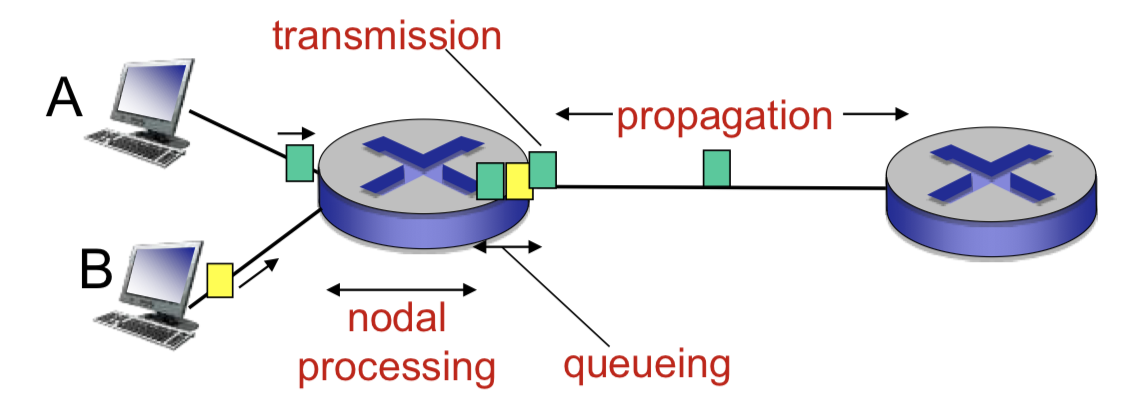
\includegraphics[width=8cm]{delay}
	\centering
	\caption{Packet Delay Algorithm Explanation}
\end{figure}
\begin{note}{Packet Delay Algorithm}
	\[ d_\text{nodal} = d_\text{proc} + d_\text{queue} + d_\text{trans} + d_\text{prop} \]
\end{note}
\subsubsection{Nodal Processing}
\[ d_\text{proc} \]
\begin{itemize}
	\item check bit errors
	\item determine output link
	\item typically < msec
\end{itemize}
\subsubsection{Queuing Delay}
\[ d_\text{queue} \]
\begin{itemize}
	\item time waiting at output link for transmission
	\item depends on congestion level of router
\end{itemize}
\subsubsection{Transmission Delay}
\[ d_\text{trans} \]
\begin{itemize}
	\item $L$: packet length (bits)
	\item $R$: link bandwidth(bps)
	\item $d_\text{trans} = \frac{L}{R}$
\end{itemize}
\subsubsection{Propagation Delay}
\[ d_\text{prop} \]
\begin{itemize}
	\item $d$: length of physical link
	\item $s$: propagation speed ($\approx2\times10^8$ m/sec)
	\item $d_\text{prop} = \frac{d}{s}$
\end{itemize}

\subsection{Throughput}
\begin{leftbar}
	Rate (bits/time unit) at which bits transferred between sender/receiver
\end{leftbar}
\begin{description}
	\item[Instantaneous:] rate at given point in time
	\item[Average:] rate over longer period of time
\end{description}
\begin{note}{Bottleneck Link}
	Link on end-end path that constrains end-end throughput
\end{note}

\subsection{Layering}
\subsubsection{Why Layering?}
Dealing with complex systems:
\begin{itemize}
	\item Explicit structure allows identification, relationship of complex system's pieces (layered \textbf{reference model} for discussion)
	\item Modularization eases maintenance, updating system
	\begin{itemize}
		\item change of implementation of layer's service transparent to rest of system
		\item e.g. change in gate procedure doesn't affect rest of system
	\end{itemize}
	\item layering considered harmful?
\end{itemize}
\subsubsection{Internet Protocol Stack}
\begin{description}
	\item[Application:] supporting network applications (FTP, SMTP, HTTP)
	\item[Transport:] process-process data transfer (TCP, UDP)
	\item[Network:] routing of datagrams from source to destination (IP, routing protocols)
	\item[Link:] data transfer between neighboring network elements (Ethernet, 802.111 (WiFi), PPP)
	\item[Physical:] bits ``on the wire''
\end{description}
\subsubsection{ISO/OSI Reference Model}
Internet stack ``missing'' these layers. These services, if needed, must be implemented in application.
\begin{description}
	\item[Application:]
	\item[Presentation:] allow applications to interpret meaning of data, e.g. encryption, compression, machine-specific conventions
	\item[Session:] synchronization, check-pointing, recovery of data exchange
	\item[Transport:]
	\item[Network:]
	\item[Link:]
	\item[Physical:]
\end{description}

\subsection{Security}
\begin{itemize}
	\item Malware can get in host from:
	\begin{description}
		\item[Virus:] self-replicating infection by receiving/executing object (e.g. e-mail attachment)
		\item[Worm:] self-replicating infection by passively receiving object that gets itself executed
	\end{description}
	\item \textbf{Spyware malware} can record keystrokes, web sites visited, upload info to collection site
	\item Infected host can be enrolled in \textbf{botnet}, used for spam. DDoS attacks
\end{itemize}
\subsubsection{DoS: Denial of Service}
\textbf{Denial of Service (DoS):} attackers make resources (server, bandwidth) unavailable to legitimate traffic by overwhelming resource with bogus traffic
\begin{enumerate}
	\item select target
	\item break into hosts around the network (botnet)
	\item send packets to target from compromised hosts
\end{enumerate}
\subsubsection{Sniffing}
\begin{itemize}
	\item broadcast media (shared Ethernet, wireless)
	\item promiscuous network interface reads/records all packets (e.g. including passwords) passing by
\end{itemize}
\subsubsection{IP Spoofing}
Send packet with false source address
	
	\section{Chapter 2}
	% !TeX spellcheck = en_US
% !TeX root = notes.tex
\subsection{Application Architectures}
\subsubsection{Client-Server}
\begin{description}
	\item[Server:] Always-on host, Permanent IP address
	\item[Clients:] Do not communicate directly with each other, May have dynamic IP addresses
\end{description}

\subsubsection{Peer-to-Peer (P2P)}
\begin{itemize}
	\item No always-on server
	\item Peers request service from other peers, provide service in return to other peers
	\item \textbf{Self Scalability} -- new peers bring new service capacity, as well as new service demands
	\item Pers are intermittently connected and change IP addresses
\end{itemize}

\begin{note}{App-layer protocol defines}
	\begin{itemize}
		\item \textbf{type of messages exchanged} -- e.g. request, response
		\item \textbf{message syntax} -- what fields in messages and how fields are delineated
		\item \textbf{message semantics} -- meaning of information in fields
		\item \textbf{rules} for when and how processes send and respond to messages
		\item \textbf{open protocols} -- defined in RFCs, allows for interoperability (e.g. HTTP, SMTP)
		\item \textbf{proprietary protocols} -- e.g. Skype
	\end{itemize}
\end{note}

\subsection{Transport Service is needed}
\begin{description}
	\item[Data Integrity:] Some programs need 100\% reliable data transfer (e.g. file transfer, web transactions), others can tolerate loss (e.g. audio)
	\item[Timing:] Some programs require low delay to be ``effective'' (e.g. online games)
	\item[Throughput:] Some programs require minimum amount of throughput to be ``effective'' (e.g. multimedia), some use whatever they have available (``elastic apps'')
	\item[Security:] Encryption, Data Integrity
\end{description}

\subsection{Transport Protocol Services}
\subsubsection{TCP}\label{sec:tcp}
\begin{description}
	\item[Reliable Transport] between sending and receiving process
	\item[Flow Control:] sender won't overwhelm receiver
	\item[Congestion Control:] throttle sender when network overloaded
	\item[Connection-Oriented:] setup required between client and server processes
	\item[Does Not Provide:] timing, minimum throughput guarantee, security
\end{description}

\subsubsection{UDP}\label{sec:udp}
\begin{description}
	\item[Unreliable Data Transfer] between sending and receiving process
	\item[Does Not Provide:] reliability, flow control, congestion control, timing, throughput guarantee, security, or connection setup
\end{description}

\subsubsection{Securing TCP}
\textbf{TCP and UDP}
\begin{itemize}
	\item no encryption
	\item cleartext passwords sent into socket traverse Internet in cleartext
\end{itemize}
\textbf{SSL}
\begin{itemize}
	\item provides encrypted TCP connection
	\item data integrity
	\item end-point authentication
\end{itemize}
\textbf{SSL is at app layer}
\begin{itemize}
	\item app use SSL libraries, that ``talk'' to TCP
\end{itemize}
\textbf{SSL socket API}
\begin{itemize}
	\item cleartext passwords sent into socket traverse Internet encrypted
\end{itemize}

\subsection{HTTP: Hypertext Transfer Protocol}\label{sec:http}
\begin{itemize}
	\item Web's application layer protocol
	\item client/server model. Client request website and server serves HTTP object in response
	\item Uses TCP
	\item HTTP is stateless. Server maintains no information about past client requests
	\item \textbf{non-persistent HTTP:} one object sent over one TCP connection, downloading multiple object required multiple connections
	\item \textbf{persistent HTTP:} multiple object sent over single TCP connection
\end{itemize}
Non-persistent HTTP issues:
\begin{itemize}
	\item requires 2 RTTs per object
	\item OS overhead for each TCP connection
	\item browsers often open parallel TCP connections to fetch referenced objects
\end{itemize}
Persistent HTTP:
\begin{itemize}
	\item server leaves connection open after sending response
	\item subsequent HTTP messages between same client/server sent over open connection
	\item client sends requests as soon as it encounters a referenced object
	\item as little as one RTT for all the referenced objects
\end{itemize}
\subsubsection{Method Types}
\textbf{HTTP/1.0:} GET, POST, HEAD (asks server to leave requested object out of response)\\
\textbf{HTTP/1.1:} GET, POST, HEAD, PUT (uploads file in entity body to path specified in URL field), DELETE (deletes file specified in the URL field)
\subsubsection{Response Codes}
\begin{description}
	\item[200 OK:] request succeeded, requested object later in this msg
	\item[301 Moved Permanently:] requested object moved, new location specified later in this msg
	\item[400 Bad Request:] request msg not understood by server
	\item[404 Not Found:] requested document not found on this server
	\item[505 HTTP Version Not Supported]
\end{description}

\subsection{Cookies}
Uses: authorization, shopping carts, recommendations, user session state (Web, email)

\subsection{Web Caches (proxy server)}
\begin{leftbar}
	\textbf{Goal:} satify client request without involving origin server
\end{leftbar}
\begin{itemize}
	\item Browsers requests object from cache, if in cache the object is sent back otherwise cache requests object from origin
	\item Cache acts as both client and server
	\item Reduce response time for client request
	\item Reduce traffic
\end{itemize}

\subsubsection{Conditional GET}
\begin{leftbar}
	\textbf{Goal:} don't send object if cache has up-to-date cached version (lower link usage)
\end{leftbar}
\begin{itemize}
	\item \textbf{Cache:} specify date of cached copy in HTTP request \texttt{If-modified-since: <date>}
	\item \textbf{Server:} response contains no object if cached copy is up-to-date: \texttt{HTTP/1.0 Not Modified}
\end{itemize}

\subsection{Electronic Mail: SMTP}\label{sec:smtp}
\textit{RFC 2821}
\begin{itemize}
	\item uses TCP to reliably transfer email message from client to server, port 25
	\item direct transfer: sending server to receiving server
	\item three phases of transfer: handshaking, transfer of messages, closure
	\item command/response interaction
	\item messages must be in 7-bit ASCII
	\item uses persistent connections
	\item requires message to be in 7-bit ASCII
	\item uses \texttt{CRLF.CRLF} to determine end of message
\end{itemize}
Difference to HTTP being, HTTP is server sending data, SMTP is client connection sending data\\
\begin{description}
	\item[SMTP:] protocol for exchanging email messages
	\item[RFC 822:] standard for text message format (To, From, Subject, Body)
\end{description}
\subsubsection{Mail Access Protocols}
\begin{leftbar}
	\textbf{SMTP:} delivery/storage to receiver's server
\end{leftbar}
\begin{description}
	\item[POP:] Post Office Protocol \textit{(RFC 1939)}: authorization, download
	\begin{itemize}
		\item POP3 is stateless across sessions
		\item Two main modes; download and delete, download and keep (allows multiple clients to read the same email)
	\end{itemize}
	\item[IMAP:] Internet Mail Access Protocol \textit{(RFC 1730)}: more features, including manipulation of stored message on server
	\begin{itemize}
		\item All messages stored on server
		\item Supports folders
		\item Keeps user state across sessions: names of folders and mappings between message IDs and folder name
	\end{itemize}
	\item[HTTP:] gmail, Hotmail, Yahoo, etc
\end{description}

\subsection{DNS: Domain Name System}\label{sec:dns}
\begin{itemize}
	\item Lookup between names (e.g. google.com) and IP addresses
	\item \textbf{Distributed Database} implemented in hierarchy of many \textbf{name servers}
	\item \textbf{Application-layer protocol:} hosts, name servers communicate to \textbf{resolve} names (address/name translation)
\end{itemize}
Why not centralize DNS? Single point of failure, traffic volume, doesn't scale
\subsubsection{DNS Services}
\begin{itemize}
	\item hostname to IP address translation
	\item host aliasing (canonical, alias names)
	\item mail server aliasing
	\item load distribution (many IP addresses correspond to one name)
\end{itemize}
\subsubsection{TLD, authoritative servers}
\textbf{top-level domain (TLD) servers:}
\begin{itemize}
	\item responsible for com, org, net, edu, aero, jos, io
	\item and top-level country domains au, uk, ca
	\item Network Solutions maintains servers for .com TLD
	\item Educause for .edu TLD
\end{itemize}
\textbf{Authoritative DNS servers:}
\begin{itemize}
	\item organization's own DNS server(s), providing authorative hostname to IP mappings for organization's named hosts
	\item can be maintained by organization or service provider
\end{itemize}
\subsubsection{Local DNS name server}
\begin{itemize}
	\item does not strictly belong to hierarchy
	\item each ISP (residential ISP, company, university) has one (also called ``default name server'')
	\item when host makes DNS query, query is sent to its local DNS server
	\begin{itemize}
		\item has local cache of recent name-to-address translation pairs (but may be out of date!)
		\item acts as proxy, forwards query into hierarchy
	\end{itemize}
\end{itemize}
\subsubsection{DNS Name Resolution}
\begin{description}
	\item[Iterated query:] contacted server replies with name of server to contact. So root dns sends the ip of the next dns server to contact
	\item[Recursive query:] puts burden of name resolution on contacted name server. So root dns server contacts the next levels down which contacts next level down.
\end{description}
\subsubsection{Caching}
Once (any) name server learns mapping, it \textbf{caches} mapping. Cache entries timeout (disappear) after some time (TTL). If name host changes IP address, the name servers might not update until TTLs expire.
\begin{leftbar}
	update/notify mechanisms proposed IETF standard RFC 2136
\end{leftbar}
\subsubsection{DNS Records}
\begin{note}{RR Format}
	\texttt{(name, value, type, ttl)}
\end{note}
\begin{description}
	\item[type=A] \texttt{name} is hostname, \texttt{value} is IP address
	\item[type=NS] \texttt{name} is domain (e.g. google.com), \texttt{value} is hostname of authoritative name server for this domain
	\item[type=CNAME] \texttt{name} is alias name for some ``canonical'' (the real) name (\texttt{www.ibm.com} is really \texttt{servereast.backup2.ibm.com}), \texttt{value} is canonical name
	\item[type=MX] \texttt{value} is name of mailserver associated with \texttt{name}
\end{description}
\subsubsection{Protocol}
Query and reply messages both follow same format
\begin{table}[H]
\centering
\caption{Protocol Layout}
\begin{tabular}{cc}
	\toprule
	2 bytes & 2 bytes \\
	\midrule
	identification & flags\\
	\# questions & \# answer RRs\\
	\# authority RRs & \# additional RRs\\
	\multicolumn{2}{c}{questions (variable \# of questions)}\\
	\multicolumn{2}{c}{answers (variable \# of RRs)}\\
	\multicolumn{2}{c}{authority (variable \# of RRs)}\\
	\multicolumn{2}{c}{additional info (variable \# of RRs)}\\
	\bottomrule
\end{tabular}
\end{table}
\subsubsection{Attacking DNS}
\textbf{DDoS attacks}
\begin{itemize}
	\item bombard root servers with traffic. Not successful to date, traffic filtering, local DNS servers cache protecting root DNS
	\item bombard TLD server. Potentially more dangerous
\end{itemize}
\textbf{Redirect Attacks}
\begin{itemize}
	\item man-in-middle (Intercept queries)
	\item DNS Poisoning (Send bogus relies to DNS server, which caches)
\end{itemize}
\textbf{Exploit DNS for DDoS}
\begin{itemize}
	\item send queries with spoofed source address: target IP
	\item requires amplification
\end{itemize}
	% !TeX spellcheck = en_US
% !TeX root = notes.tex
\section{Lecture 3: Bitcoin, Cryptocurrencies Blockchain Technology}
\subsection{Sybil Attack}
\begin{itemize}
	\item The Sybil attack in computer security is an attack wherein a reputation system is subverted by forging identities in peer-to-peer networks.
	\item Creates a large number of false identities in order to flood the network and take it over.
	\item Named after the subject of the book \textbf{Sybil}, a case study of a woman diagnosed with multiple personality disorder
	\item Such false identities are called \textbf{``Sybils''}, in the context of P2P systems
	\item One approach to preventing these “Sybil attacks” is to have a trusted agency certify identities.
	\item Or \textbf{``Sockpuppets''} in the context of the Internet, e.g. to manipulate public opinion
	\begin{leftbar}
		``... referred to a false identity assumed by a member of an Internet community who spoke to, or about, themselves while pretending to be another person. `The term now includes other misleading uses of online identities, such as those created to praise, defend or support a person or organization, to manipulate public opinion, or to circumvent a suspension or ban from a website''\\
		- Wikipedia
	\end{leftbar}
\end{itemize}

\subsection{Decentralized Consensus in Bitcoin}
\begin{itemize}
	\item Bitcoin achieves consensus by replacing \textbf{one node (or one IP address) one vote}, with \textbf{one CPU one vote}
	\item Bitcoin mining uses mostly ASICs and GPUs, not CPUs
	\item Consensus is achieved by a (probabilistic) majority vote, based on computing power
	\begin{itemize}
		\item Attacker needs > 50\% of combined computing power in order to cheat with high probability
		\item This is harder to achieve than controlling more than half of the nodes
		\item It's relatively easy to spin up a few thousand VMs as nodes, compared to controlling >50\% of Bitcoin's mining compute power
	\end{itemize}
	\item Bitcoin combines a \textbf{proof-of-work mechanism} (based on Hashcash), combined with a clever incentive mechanism $\rightarrow$ Nodes get paid to do the right thing, i.e. checking and confirming valid transactions via ``mining''
\end{itemize}

\section{Lecture 3: Bitcoin}
\begin{itemize}
	\item Complete transaction history is stored in public ledger (blockchain), stored by nodes in P2P network
	\item New transactions are created off-line, and then broadcast is P2P network
	\item Nodes validate and relay transactions (if valid)
	\item Nodes add new transactions (not part of blockchain yet) to a \textbf{transaction pool}
	\item Nodes combine transactions in pool to a block, and try to solve the corresponding proof-of-work puzzle, to ``confirm'' the block
	\item Node that finds solution first broadcasts block with solution in the network (Winning node selection is probabilistic, with probability propertional to computing power)
	\item Nodes check solution, and if OK, add new block to their local copy of blockchain
	\item All nodes who were working on solving the old puzzle, immediately start working on a new block
	\begin{itemize}
		\item Everybody always works on the longest chain
		\item Convergence to longest chain provides consensus
		\item Forks happen but are resolved by (computational) majority vote
	\end{itemize}
\end{itemize}
\begin{note}{Bitcoin Components}
	\begin{itemize}
		\item Bitcoin Network
		\item Bitcoin Identities/Addresses
		\item Bitcoin Transactions
		\item Bitcoin Scripting Language
		\item Blocks
		\item Proof-of-work, Hash puzzles, Mining
		\item Consensus
	\end{itemize}
\end{note}

\subsection{Bitcoin Network}
Transactions are broadcast in the Bitcoin network, consisting of ``full'' Bitcoin nodes ($\approx$10,000)
\begin{itemize}
	\item Best-effort (asynchronous, unreliable), it's enough if only some nodes get the message
	\item It's easy to join the Bitcoin Network, just download and run the client (Bitcoin is a \textbf{permissionless, public} blockchain, anyone can join)
\end{itemize}
Network is unstructured P2P network (random topology)
\begin{itemize}
	\item Similar to Gnutella (a P2P system from a long time ago)
	\item Overlay network, TCP, port 8333
	\item Messages are flooded
	\item All nodes are equal, no hierarchy
	\item Nodes can join at any time
	\item Node is `forgotten' if it does not respond for more than 3 hours
	\item Network is very simple and robust, e.g. to churn, but not very efficient
\end{itemize}
\begin{note}{Bitcoin Network Nodes}
	\begin{itemize}
		\item Check validity of transactions
		\item Relay transactions in the network via flooding
		\item Mining (proof-of-work puzzles)
		\item Validate and forward confirmed blocks (Add them to local copy of blockchain)
	\end{itemize}
\end{note}
\subsection{Bitcoin Identity and Addresses}
Users are represented by their Public Key addresses (hash), called \textbf{Bitcoin Addresses}, which serve as a pseudonyms
\begin{itemize}
	\item An address is a \textbf{160 bit} value, and is computed as follows
	\item RIPEMD160 hash of SHA-256 hash of ECDSA Public Key
	\item This is a ``Pay-to-pubkey-hash (P2PKH)'' address, encoding starts with ``1''
\end{itemize}
When spending a coin, spender needs to proof ownership of coin by providing a valid digital signature on the spend transaction (i.e. proving ownership of corresponding private key)\\
How can digital signatures be verified?
\begin{itemize}
	\item We need public key, not just hash of public key
	\item Spender of coin needs to provide both valid signature AND public key
	\item How do we know the provided public key is authentic $\rightarrow$ Hash it, and compare with Bitcoin address, which is the hash of public key
\end{itemize}
Bitcoin also supports \textbf{Pay to script hash (P2SH)} addresses
\begin{itemize}
	\item Allow transactions to be sent to a \textbf{script hash} instead of a public key hash (Address encoding starts with a `3' instead of `1')
	\item To spend bitcoins sent via P2SH, the recipient must provide a script matching the script hash and data which makes the script evaluate to true
	\item Allows more complex transactions (\textbf{smart contracts}), e.g. transaction outputs that require multiple signatures (multisig), or transaction puzzle, ...
\end{itemize}
\begin{note}{Bitcoin Address Encoding}
	Bitcoin uses Base58 encoding (binary-to-text encoding). Similar to Base64 encoding, but without some characters. Rationale, as explained in original bitcoin client source code:
	\begin{code}
		// Why base-58 instead of standard base-64 encoding?\\
		// - Don't want 0OIL characters that look like the same in some fonts and\\
		//   could be used to create visually identical looking account numbers.\\
		// - A string with non-alphanumeric characters is not as easily accepted as an account nbr.\\
		// - E-mail usually won't line-break if there's no punctuation to break at.\\
		// - Doubleclicking selects the whole number as one word if it's all\\alphanumeric.
	\end{code}
	Bitcoin also adds 4 byte checksum to addresses
\end{note}
\subsubsection{Bitcoin Address -- Balance}
\begin{itemize}
	\item The ``balance'' of an address is the total of unspent transaction outputs (UTXO) sent to the address.
	\item ``There are no accounts or balances in bitcoin; there are only unspent transaction outputs (UTXO) scattered in the blockchain''
	\item A user typically has many different addresses, all managed by the ``wallet'' software
	\item The wallet ``balance'' is the sum of all unspent transaction outputs of all addresses owned by the user
\end{itemize}
\subsection{Bitcoin Transactions}
\begin{itemize}
	\item Transaction are created off-line (No need to be connected to Bitcoin network for this)
	\item Transactions are broadcast in Bitcoin P2P network
	\item Nodes check validity, and relay transaction (flooding)
	\item Nodes add to new transactions to a block and try to solve hash puzzle
	\item A block with a solved puzzle is ``confirmed'', and broadcast in the network, and added to the blockchain of each node
	\item Contains:
	\begin{itemize}
		\item Inputs (any number $\geq0$)
		\item Outputs (any number > 0)
		\item Digital signatures of input coin owners (Typically for \textbf{P2PKH} transactions)
		\item Input needs to be completely consumed (With exception of Transaction Fee)
	\end{itemize}
\end{itemize}
\subsubsection{Basic Transaction Types}
\begin{itemize}
	\item Common Transaction
	\begin{itemize}
		\item 1 input
		\item 1 ``normal'' output
		\item 1 change output (back to owner)
		\subitem Create new ``Change Address'' to maintain ``anonymity''
	\end{itemize}
	\item Aggregating Transaction
	\begin{itemize}
		\item Multiple inputs
		\item 1 output
	\end{itemize}
	\item Distributing Transaction
	\begin{itemize}
		\item 1 input
		\item Multiple outputs
	\end{itemize}
	\item ``Coinbase Transaction''
	\begin{itemize}
		\item 0 input, 1 outputs
		\item Freshly created (``minted'') coins
		\item Miner gets this as a reward for solving Hash puzzle (and thereby confirming block)
		\item First transaction in every block
	\end{itemize}
\end{itemize}

\subsection{Bitcoin Scripts}
\begin{itemize}
	\item Two types of Bitcoin scripts to validate transactions
	\begin{itemize}
		\item a locking script (Typically \textbf{ScriptPubKey})
		\item and an unlocking script (Typically \textbf{ScriptSig})
	\end{itemize}
	\item A locking script is a condition placed on an output
	\item It specifies the conditions that must be met to spend or consume the output in the future
	\begin{itemize}
		\item Typically a \textbf{valid digital signature} of the claimed owner
		\item Can be other things, to implement basic `smart contracts'
	\end{itemize}
\end{itemize}
\subsubsection{Bitcoin Scripting Language ``Script''}
\begin{itemize}
	\item Allows to program conditions required for the spending of Bitcoins (``Programmable Money'')
	\item \textbf{Script} is a simple, stack based language
	\item Not Turing complete (e.g. no loops)
	\item Scripts are guaranteed to terminate after a fixed number of steps, e.g. no infinite loops
	\item Why is this a good thing?
	\begin{itemize}
		\item Avoids potential denial of service attacks on nodes, ``logic bombs''
		\item Remember: Every node runs all scripts to validate all transactions (BTW, this severely limits scalability of Bitcoin)
	\end{itemize}
	\item In contrast, Ethereum has a Turing complete scripting language
	\subitem Solves DoS attack problem by putting a price on script computation (`Gas')
\end{itemize}

\subsection{Blocks}
\begin{itemize}
	\item Transactions are grouped into blocks
	\subitem This is an optimization. Confirming individual transactions and adding them to the blockchain would be possible, but very inefficient
	\item Transactions are stored in a Merkle Tree, with the Merkle Root (Tx\_Root) stored in the block header
	\item Once confirmed (via solving hash puzzle), a block is added to the blockchain
	\item The `Nonce' is the solution of the hash puzzle
\end{itemize}
\begin{figure}[H]
	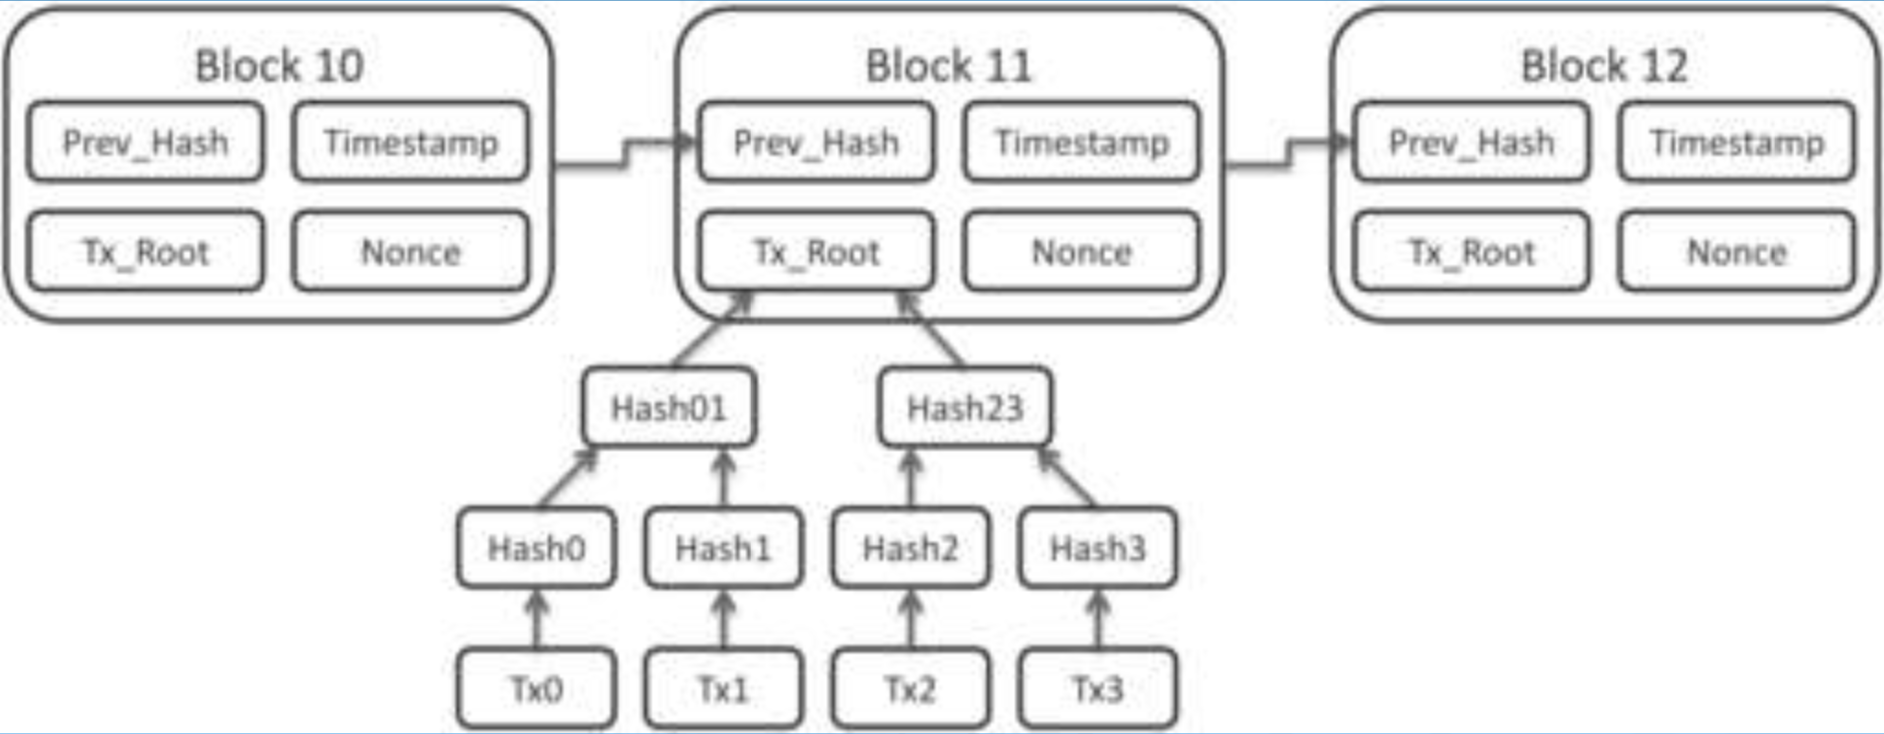
\includegraphics[width=\linewidth]{blockStructure}
	\centering
	\caption{Block Structure}
\end{figure}
\subsubsection{How are blocks added to the Blockchain?}
\begin{itemize}
	\item Multiple nodes (miners) are working towards solving the hash puzzle for a new block
	\subitem miners are probably working on different version of blocks, depending on content on their transaction pool
	\item First node who solves puzzle, broadcasts new block with solution (nonce) in the Bitcoin P2P network
	\begin{itemize}
		\item Choice of winning node is random (probabilistic)
		\item Probability of success is proportional to computing power of miner
	\end{itemize}
	\item ``Block Height'' is sequence number of blocks
	\item Other nodes check if solution is correct, and if so, add block to their local copy of the blockchain, and forward new block to other nodes
\end{itemize}

\subsection{Bitcoin Mining}
\begin{itemize}
	\item At the current level of difficulty, solving Bitcoin hash puzzles is hard and expensive
	\item Mostly ASICs based, some GPUs
	\item Total hash rate of entire Bitcoin network $\approx25\times10^{18}$H/s
	\item Hash rate of an Intel i7 CPU $\approx10$MH/s
	\subitem Need > 10,000,000 laptops to be able to mine one block per year on average
	\item Finite amount of BTC $\approx$21 Million
	\item Bitcoin is deflationary (value increases, people are potentially hoarding Bitcoin)
\end{itemize}
\subsubsection{Mining Incentive/Reward}
\begin{itemize}
	\item Transaction Fees
	\begin{itemize}
		\item Difference between total input and total output value of transaction
		\item Optional, but miners prioritize inclusion of transactions into blocks based on fees (Like giving a tip)
	\end{itemize}
	\item Block Reward
	\begin{itemize}
		\item For each solved puzzle (confirmation of block), miner currently gets freshly minted 12.5 BTC
		\item ``Coinbase transaction'' ($1^{st}$ transaction in each block)
		\item This is the only way in which coins are generated in Bitcoin
		\item Reward halved every 4 years (initially 50 BTC)
		\item Essentially no more Block Reward in 2040
	\end{itemize}
\end{itemize}

\subsection{Consensus}
\begin{itemize}
	\item Blockchain forks can happen, e.g. due to race conditions and variable latency in Bitcoin network (\textit{two nodes might find a solution to the puzzle at almost the same time}), or due to double spend attempt
	\item Nodes converge on one chain, they all aim to work on the longest (main) chain, and eventually one chain wins
	\item Incentive to work on the longest chain (Block Reward and TX fees can only be spent if block remains in the longest chain (need a certain number of \textbf{confirmations}, i.e. blocks added))
	\item Block on discontinued branches are called ``orphaned blocks''
	\item Heuristic
	\subitem Transactions are considered ``confirmed'' if they are in a block that has at least 6 blocks added to the chain (i.e. 6 confirmation) \textit{(There is nothing special about the number 6)}
	\item This means if someone wanted to reverse a transaction, they would have to go back 6 blocks, and re-do all the hash puzzles, before another nodes adds a new block at the end of chain (Practically impossible, unless attacker hash more than 50\% of computing power of entire network)
	\item Other types of attacks:
	\begin{itemize}
		\item Publish an invalid transaction, e.g. trying to spend coins that he does not own (no valid signature). Honest nodes would reject the transaction
		\item Double spend attack. Cause a fork in the chain, majority vote will guarantee that only one chain will exist
		\item Launch DoS attack against
	\end{itemize}
	\item With more than 50\% computing power, more beneficial to play by the rules and gain Block Rewards
\end{itemize}
	
	\section{Chapter 3}
	% !TeX spellcheck = en_US
% !TeX root = notes.tex
\subsection{Transport vs. Network Layer}
\begin{description}
	\item[Network Layer:] logical communication between hosts
	\item[Transport Layer:] logical communication between processes; relies on, enhances, network layer services
\end{description}

\subsection{Multiplexing/demultiplexing}
\subsubsection{How demultiplexing works}
\begin{itemize}
	\item host receives IP datagrams
	\begin{itemize}
		\item each datagram as source IP address, destination IP address
		\item each datagram carries one transport-layer segment
		\item each segment has source, destination port number
	\end{itemize}
	\item host uses \textbf{IP addresses and port numbers} to direct segment to appropriate socket
\end{itemize}\newpage
\textbf{Connectionless Demultiplexing}
\begin{leftbar}
	A UDP socket needs to have a local port number assigned to it (both client and server)
\end{leftbar}
\textbf{Connection-oriented demux}
\begin{leftbar}
	TCP socket identified by 4-tuple: \textbf{(source IP address, source port number, dest IP address, dest port number)}
\end{leftbar}

\subsection{UDP}
\begin{table}[H]
	\centering
	\caption{UDP Segment Header}
	\begin{tabular}{cc}
		\toprule
		\multicolumn{2}{c}{32 bits}\\
		\midrule
		source port \# & dest port \#\\
		length & checksum\\
		\multicolumn{2}{c}{application data (payload)}\\
		\bottomrule
	\end{tabular}
\end{table}
\subsubsection{UDP Checksum}
\textbf{Sender:}
\begin{itemize}
	\item treat segment contents, including header fields, as sequence of 16-bit integers
	\item checksum: addition (one's complement sum) of segment contents
	\item sender puts checksum value into UDP checksum field
\end{itemize}
\textbf{Receiver:}
\begin{itemize}
	\item compute checksum of received segment
	\item check if computed checksum equals checksum field value
\end{itemize}

\subsection{Pipelined Protocols}
\begin{leftbar}
	\textbf{Pipelining:} sender allows multiple, "in-flight", yet-to-be-acknowledged packets. Range of sequence numbers must be increased, buffering at sender and/or receiver.
\end{leftbar}
\subsubsection{Go-Back-N}
\begin{itemize}
	\item sender can have up to$N$ unacked packets in pipeline
	\item receiver only sends \textbf{cumulative ack}. Doesn't ack packet if there's a gap
	\item sender has timer for oldest unacked packet. When timer expires, retransmit all unacked packets
\end{itemize}
\subsubsection{Selective Repeat}
\begin{itemize}
	\item sender can have up to $N$ unacked packets in pipeline
	\item receiver sends \textbf{individual ack} for each packet
	\item sender maintains timer for each unacked packet. When timer expires, retransmit only that unacked packet
\end{itemize}
	% !TeX spellcheck = en_US
% !TeX root = notes.tex
\subsection{TCP Segment Structure}
\begin{leftbar}
	TCP contains a handshake to make sure both ends are willing to open a connection
\end{leftbar}
\begin{table}[H]
	\centering
	\caption{TCP Segment Structure}
	\begin{tabular}{cc}
		\toprule
		\multicolumn{2}{c}{32 bits}\\
		\midrule
		source port \# & dest port \#\\
		\multicolumn{2}{c}{sequence number}\\
		\multicolumn{2}{c}{acknowledgment number}\\
		(head len, not used, UAPRSF) & receive window\\
		checksum & urg data pointer\\
		\multicolumn{2}{c}{options (variable length)}\\
		\multicolumn{2}{c}{application data (variable length)}\\
		\bottomrule
	\end{tabular}
\end{table}
\begin{leftbar}
	\textbf{sequence number, acknowledgment number:} counting by bytes of data (not segments)\\
	\textbf{U:} urgent data (generally not used)\\
	\textbf{A:} ACK \# valid\\
	\textbf{P:} push data now (generally not used)\\
	\textbf{RSF:} RST, SYN, FIN; connection established (setup, teardown commands)\\
	\textbf{checksum:} Internet checksum (as in UDP)\\
	\textbf{receive window:} \# bytes receiver willing to accept
\end{leftbar}
\begin{description}
	\item[Sequence Numbers:] byte stream ``number'' of first byte in segment's data
	\item[Acknowledgements:] sequence \# of next byte expected from other side, cumulative ACK
\end{description}
\subsubsection{TCP Round Trip Time, Timeout}
$$ E = (1-\alpha)\times E+\alpha\times\textit{SampleRTT} $$
Where $E$ is EstimatedRTT. Influence of past sample decreases exponentially fast. Typical value: $\alpha = 0.125$
$$ \textit{TimeoutInterval} = E + 4\times\textit{DevRTT} $$
Where \textit{DevRTT} is the safety margin ($ \textit{DevRTT} = (1-\beta)\times\textit{DevRTT}+\beta\times\mid\textit{SampleRTT}-E\mid $(typically, $\beta=0.25$))
\subsubsection{TCP Flow Control}
\begin{itemize}
	\item receiver ``advertises'' free buffer space by including \texttt{rwnd} value in TCP header of receiver-to-sender segments
	\begin{itemize}
		\item \texttt{RcvBuffer} size set via socket options (typical default is 4096 bytes)
		\item many operating systems autoadjust \texttt{RcvBuffer}
	\end{itemize}
	\item sender limits amount of unacked (``in-flight'') data to receiver's \texttt{rwnd} value
	\item guarantees receive buffer will not overflow
\end{itemize}
\subsubsection{Closing}
\begin{itemize}
	\item client, server each close their side of connection (send TCP segment with FIN bit 1)
	\item respond to received FIN with ACK (on receiving FIN, ACK can be combined with own FIN)
	\item simultaneous FIN exchanges can be handled
\end{itemize}

\subsection{TCP Congestion Control}
\textbf{Approach:} sender increases transmission rate (window size), probing for usable bandwidth, until loss occurs
\begin{description}
	\item[Additive Increase:] increase \texttt{cwnd} by 1 MSS every RTT until loss detected
	\item[Multiplicative Decrease:] cut \texttt{cwnd} in half after loss
\end{description}

\subsection{Fairness}
TCP is fair because:
\begin{itemize}
	\item additive increase gives slope of 1, as throughput increases
	\item multiplicative decrease decreases throughput proportionally
\end{itemize}
UDP is not fair:
\begin{itemize}
	\item do not want rate throttled by congestion control
	\item send audio/video at constant rate, tolerate packet loss
\end{itemize}

\subsection{Explicit Congestion Notification}
Network-assisted Congestion Control:
\begin{itemize}
	\item two bits in IP header (ToS field) marked by \textbf{network router} to indicated congestion
	\item congestion indication carried to receiving host
	\item receiver (seeing congestion indication in IP datagram) sets ECE bit on receiver-to-sender ACK segment to notify sender of congestion
\end{itemize}
	
	\section{Chapter 4}
	% !TeX spellcheck = en_US
% !TeX root = notes.tex
\subsection{Network Layer}
\begin{itemize}
	\item transport segment from sending to receiving host
	\item on sending side encapsulates segments into datagrams
	\item on receiving side, delivers segments to transport layer
	\item network layer protocols in \textbf{every} host, router
	\item router examines header fields in all IP datagrams passing through it
\end{itemize}
\subsubsection{Network Layer Functions}
\begin{description}
	\item[Forwarding:] move packets from router's input to appropriate router output
	\item[Routing:] determine route taken by packets from source to destination \textit{(routing algorithms)}
\end{description}
\subsubsection{Data Plane, Control Plane}
\textbf{Data Plane}
\begin{itemize}
	\item local, per-router function
	\item determines how datagram arriving on router input port is forwarded to router output port
	\item forwarding function
\end{itemize}
\textbf{Control plane}
\begin{itemize}
	\item network-wide logic
	\item determines how datagram is routed among routers along end-end path from source host to destination host
	\item two control-plane approaches:
	\begin{description}
		\item[Traditional Routing Algorithms:] implemented in routers
		\item[Software-defined networking (SDN):] implemented in (remote) servers
	\end{description}
\end{itemize}

\subsection{Router Forwarding}
\begin{description}
	\item[Destination-based forwarding:] forward based only on destination IP address (traditional)
	\item[Generalized forwarding:] forward based on any set of header field values
\end{description}
\subsubsection{Destination-based forwarding}
A link interface is assigned to a range of destination address ranges\newpage
\begin{note}{Longest Prefix Matching}
	When looking for forwarding table entry for given destination address, use \textbf{longest} address prefix that matches destination address. Longest prefix matching: often performed using ternary content addressable memories (TCAMs). Cisco Catalyst can hold up $\approx$1M routing table entries in TCAM.
\end{note}
\begin{description}
	\item[Content Addressable:] present address to TCAM; retrieve address in one clock cycle, regardless of table size
\end{description}
\subsubsection{Switching Fabrics}
\begin{itemize}
	\item transfer packet from input buffer to appropriate output buffer
	\item switching rate: rate at which packets can be transfered from inputs to outputs (often measured as multiple of input/output line rate, $N$ inputs: switching rate $N$ times line rate desirable)
	\item three types of switching fabrics
\end{itemize}
\begin{figure}[H]
	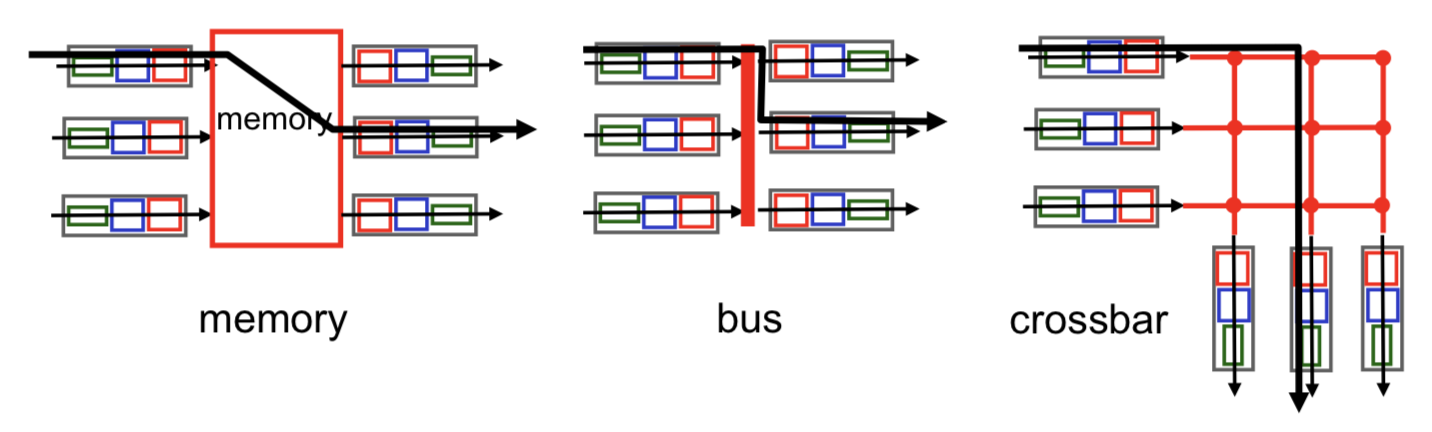
\includegraphics[width=\linewidth]{switching}
	\centering
	\caption{Different Types of Switching Fabrics}
\end{figure}
\textbf{Switching via Memory}
\begin{itemize}
	\item traditional computes with switching under direct control of CPU
	\item packet copied to system's memory
	\item speed limited memory bandwidth (2 bus crossing per datagram)
\end{itemize}
\textbf{Switching via a Bus}
\begin{itemize}
	\item datagram from input port memory to output port memory via a shared bus
	\item \textbf{bus contention:} switching speed limited by bus bandwidth
	\item 32 Gbps bus, Cisco 5600: sufficient speed for access and enterprise routers
\end{itemize}
\textbf{Switching via Interconnection Network}
\begin{itemize}
	\item overcome bus bandwidth limitations
	\item banyan networks, crossbar, other interconnection nets initially developed to connect processors in multiprocessor
	\item advanced design: fragmenting datagram into fixed length cells, switch cells through the fabric
	\item Cisco 12000: switches 60 Gbps through the interconnection network
\end{itemize}
\subsubsection{Input port queuing}
\begin{itemize}
	\item fabric slower than input ports combined $\rightarrow$ queuing may occur at input queues (queuing delay and loss due to input buffer overflow)
	\item \textbf{Head-of-the-Line (HOL) blocking:} queued datagram at front of queue prevents others in queue from moving forward
\end{itemize}
\subsubsection{Output ports}
\begin{itemize}
	\item \textbf{Buffering} required from fabric faster rate (Datagram (packets) can be lost due to congestion, lack of buffers)
	\item \textbf{Scheduling} datagrams (Priority scheduling -- who gets best performance, network neutrality)
\end{itemize}
\begin{note}{How much buffering?}
	RFC 3439 rule of thumb: average buffering equal to ``typical'' RTT (say 250 msec) times link capacity C (e.g. C = 10 Gbps link, 2.5 Gbit buffer). Recent recommendation with $N$ flows, buffering equal to $$\frac{RTT\times C}{\sqrt{N}}$$
\end{note}
\subsubsection{Scheduling Mechanisms}
\begin{description}
	\item[Scheduling:] choose next packet to send on link
	\item[FIFO scheduling:] send in order of arrival to queue
	\begin{description}
		\item[discard policy:] if packet arrives to full queue, who to discard
		\begin{description}
			\item[tail drop:] drop arriving packet
			\item[priority:] drop/remove on priority basis
			\item[random:] drop/remove randomly
		\end{description}
	\end{description}
	\item[priority scheduling:] send highest priority queued packet. Multiple \textit{classes}, with different priorities (class may depend on marking or other header info, e.g. IP source/dest, port number, etc)
	\item[RR scheduling:] multiple classes. Cyclically scan class queues, sending one complete packet from each class (if available)
	\item[WFQ scheduling:] generalized Round Robin. Each class gets weighted amount of service in each cycle
\end{description}

\subsection{IP}
\subsubsection{IP Datagram Format}
\begin{figure}[H]
	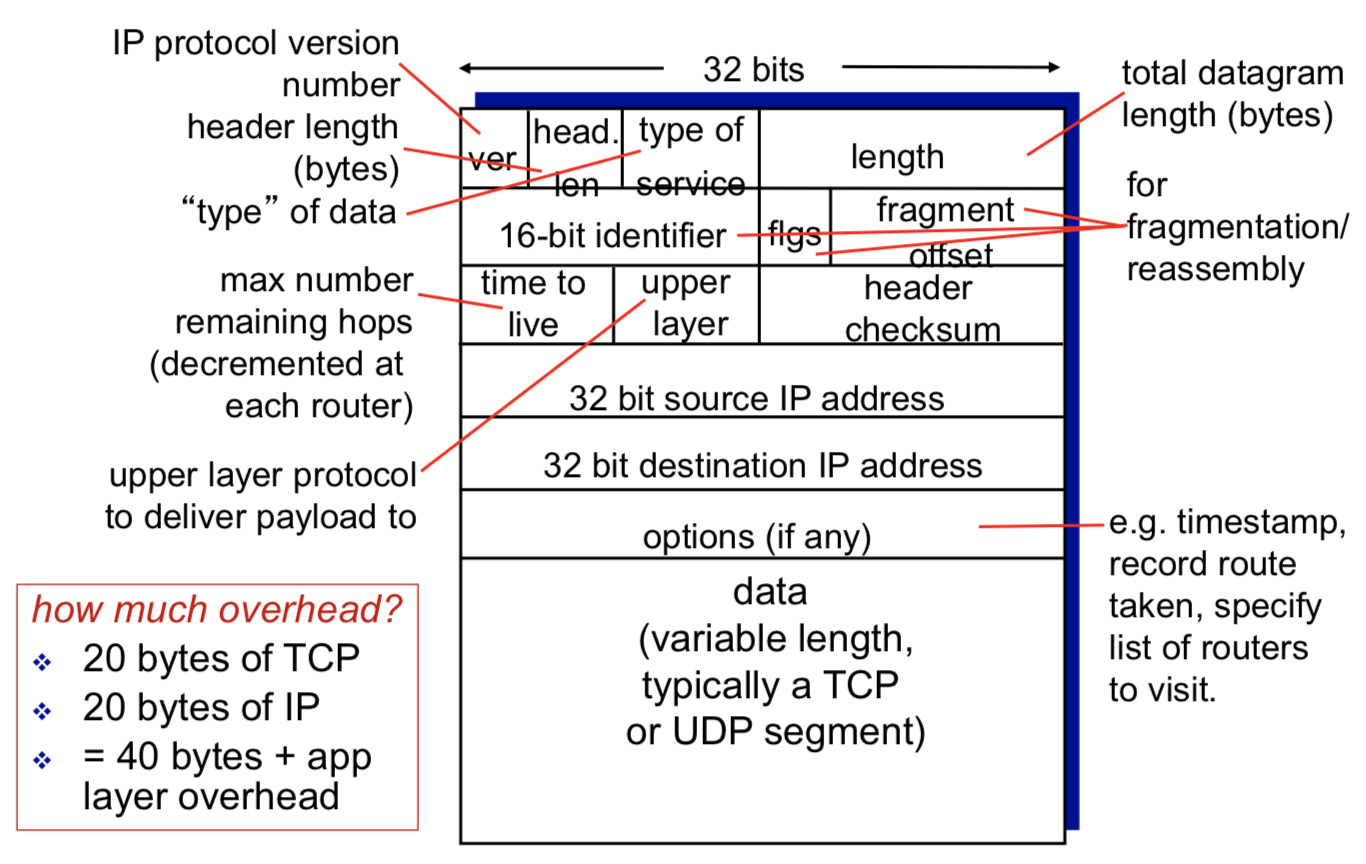
\includegraphics[width=\linewidth]{ip}
	\centering
	\caption{IP Datagram Format}
\end{figure}
\subsubsection{IP Fragmentation, Reassembly}
Large IP datagram divided (``fragmented'') within net
\begin{itemize}
	\item one datagram becomes several datagrams
	\item ``reassembled'' only at final datagrams
	\item IP header bits used to identify, order related fragments
\end{itemize}
\subsubsection{IP Addressing}
\begin{description}
	\item[IP Address:] 32-bit identifier for host, router interface
	\item[interface:] connection between host/router and physical link. Router's typically have multiple interfaces
\end{description}
\subsubsection{Subnets}
\textbf{Subnet part} -- high order bits. \textbf{Host part} -- low order bits
\begin{itemize}
	\item device interfaces with same subnet part of IP address
	\item can physically reach each other \textbf{without intervening router}
	\item to determine the subnets, detach each interface from its host or router, creating islands of isolated networks
	\item each isolated network is called a \textbf{subnet}
\end{itemize}
CIDR: Classless InterDomain Routing
\begin{itemize}
	\item subnet portion of address of arbitrary length
	\item address format: \texttt{a.b.c.d/x}, where \texttt{x} is \# bits in subnet portion of address
\end{itemize}
\subsubsection{DHCP: Dynamic Host Configuration Protocol}
\begin{leftbar}
	\textbf{Goal:} allow host to \textit{dynamically} obtain its IP address from network server when it joins network
\end{leftbar}
\begin{itemize}
	\item can renew its lease on address in use
	\item allows reuse of addresses (only hold address while connected)
	\item support for mobile users who want to join network (more shortly)
\end{itemize}
DHCP overview:
\begin{itemize}
	\item host broadcasts ``DHCP discover'' msg \textit{[optional]}
	\item DHCP server responds with ``DHCP offer'' msg \textit{[optional]}
	\item host requests IP address: ``DHCP request'' msg
	\item DHCP server sends address: ``DHCP ack'' msg
\end{itemize}
DHCP can return more than just allocated IP address on subnet:
\begin{itemize}
	\item address of first-hop router for client
	\item name and IP address of DNS server
	\item network mask (indicating network versus host portion of address)
\end{itemize}
\subsubsection{ICANN}
\begin{itemize}
	\item allocates addresses
	\item manages DNS
	\item assigns domain names, resolves disputes
\end{itemize}
\subsubsection{NAT}
All datagrams \textbf{leaving} local network have \textbf{same} single source NAT IP address
\begin{leftbar}
	\textbf{Motivation:} local network uses just one IP address as far as outside world is concerned
\end{leftbar}
\begin{itemize}
	\item range of addresses not needed from ISP: just one IP address for all devices
	\item can change addresses of devices in local network without notifying outside world
	\item can change ISP without changing addresses of devices in local network
	\item devices inside local net not explicity addressable, visible by outside world (a security plus)
\end{itemize}
\textbf{Implementation:} NAT router must
\begin{description}
	\item[Outdoing datagrams: replace] (source IP address, port \#) of every outgoing datagram to (NAT IP address, new port \#) ... remote clients/servers will respond using (NAT IP address, new port \#) as destination address
	\item[Remember (in NAT translation table)] every (source IP address, port \#) to (NAT IP address, new port \#) translation pair
	\item[Incoming datagrams: replace] (NAT IP address, new port \#) in destination fields of every incoming datagram with corresponding (source IP address, port \#) stored in NAT table
\end{description}
\begin{itemize}
	\item 16-bit port-number field: 60,000 simultaneous connections with a single LAN-side address
	\item NAT is controversial:
	\begin{itemize}
		\item routers should only process up to layer 3
		\item address shortage should be solved by IPv6
		\item violates end-to-end argument (NAT possibility must be taken into account by app designers, e.g. P2P applications)
		\item NAT traversal: what if client wants to connect to server behind NAT?
	\end{itemize}
\end{itemize}
\subsubsection{IPv6}
\begin{leftbar}
	32-bit address space soon to be completely allocated
\end{leftbar}
Additionally:
\begin{itemize}
	\item header format helps speed processing/forwarding
	\item header changes to facilitate QoS
\end{itemize}
\textbf{IPv6 datagram format:}
\begin{itemize}
	\item fixed-length 40 byte header
	\item no fragmentation allowed
\end{itemize}
\subsubsection{IPv6 Datagram Format}
\begin{description}
	\item[Priority:] identify priority among datagrams in flow
	\item[Flow Label:] identify datagrams in same ``flow'' (concept of ``flow'' not well defined)
	\item[Next Header:] identify upper layer protocol for data
\end{description}
\begin{table}[H]
	\centering
	\caption{IPv6 Format}
	\begin{tabular}{cccc}
		\toprule
		\multicolumn{4}{c}{32 bits}\\
		\midrule
		version & pri & \multicolumn{2}{c}{flow label}\\
		\multicolumn{2}{c}{payload len} & next hdr & hop limit\\
		\multicolumn{4}{c}{source address (128 bits)}\\
		\multicolumn{4}{c}{destination address (128 bits)}\\
		\multicolumn{4}{c}{data}\\
		\bottomrule
	\end{tabular}
\end{table}
\subsubsection{Other changes from IPv4}
\begin{description}
	\item[checksum:] removed entirely to reduce processing time at each hop
	\item[options:] allowed, but outside of header, indicated by ``Next Header'' field
	\item[ICMPv6:] new version of ICMP (additional message types e.g. ``Packet Too Big'', multicast group management functions)
\end{description}
\subsubsection{Transition from IPv4 to IPv6}
\begin{itemize}
	\item not all routers can be upgraded simultaneously (no ``flag days'', how will network operate with mixed IPv4 and IPv6 routers)
	\item \textbf{tunneling:} IPv6 datagram carried as \textit{payload} in IPv4 datagram among IPv4 routers
\end{itemize}

\subsection{Generalized Forwarding and SDN}
Each router contains a \textbf{flow table} that is computed and distributed by a logically centralized routing controller
\subsubsection{OpenFlow data plane abstraction}
\textbf{Flow:} defined by header fields\\
\textbf{Generalized Forwarding:} simple packet-handling rules
\begin{description}
	\item[Pattern:] match values in packet header fields
	\item[Actions:] for matched packet: drop, forward, modify, matched packet and send matched packet to controller
	\item[Priority:] disambiguate overlapping patterns
	\item[Counters:] \# bytes and \# packets
\end{description}
\begin{figure}[H]
	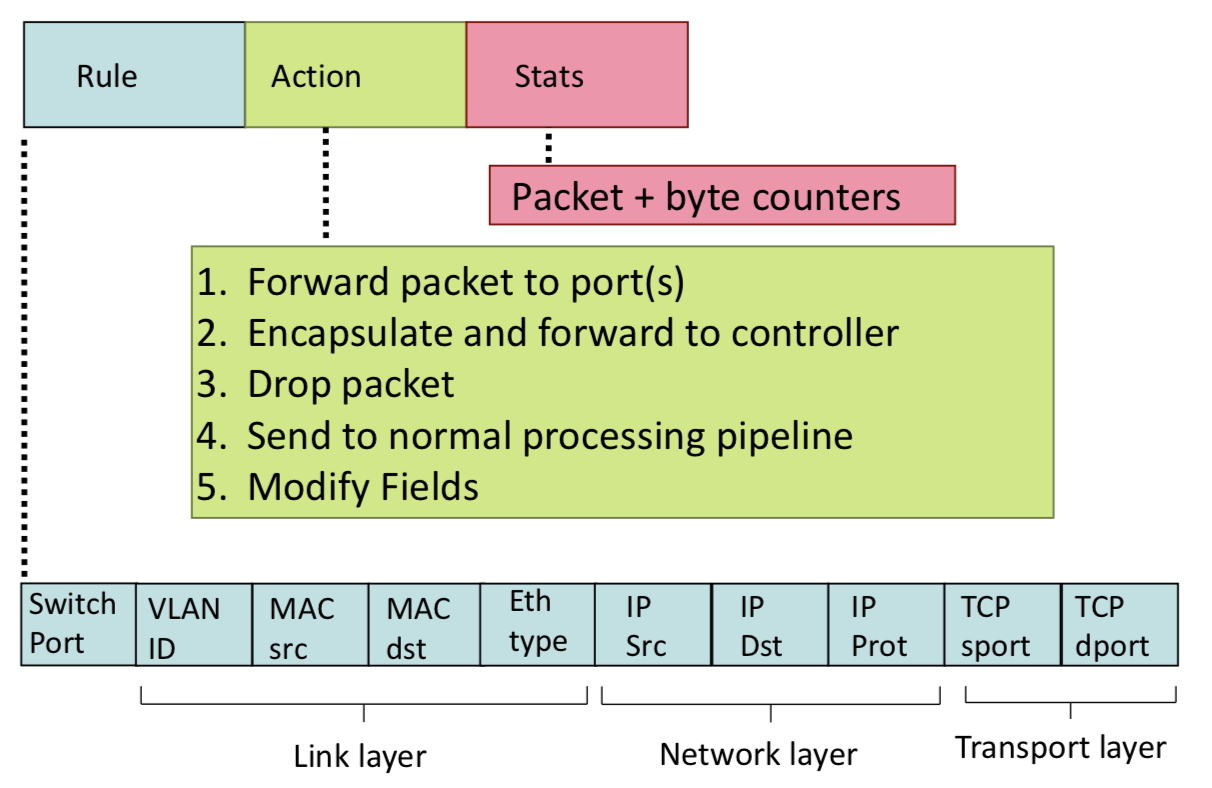
\includegraphics[width=\linewidth]{flow}
	\centering
	\caption{Flow Table Entries}
\end{figure}
\subsubsection{OpenFlow Abstraction}
\begin{itemize}
	\item \textbf{Match+Action:} unifies different kinds of devices
	\item Router
	\begin{description}
		\item[match:] longest destination IP prefix
		\item[action:] forward out a link
	\end{description}
	\item Switch
	\begin{description}
		\item[match:] destination MAC address
		\item[action:] forward or flood
	\end{description}
	\item Firewall
	\begin{description}
		\item[match:] IP addresses and TCP/UDP port numbers
		\item[action:] permit or deny
	\end{description}
	\item NAT
	\begin{description}
		\item[match:] IP address and port
		\item[action:] rewrite address and port
	\end{description}
\end{itemize}
	
	\section{Chapter 5}
	% Add BGP, OSPF, IS-IS, RIP (know if they are inter-AS or intra-AS, link-state or distance-vector)
	% !TeX spellcheck = en_US
% !TeX root = notes.tex
\subsection{Control Plane}
Two approaches to structuring network control plane:
\subsubsection{Per-router control plane}
\begin{leftbar}
	Individual routing algorithm components \textbf{in each and every router} interact with each other in control plane to compute forwarding tables
\end{leftbar}
\subsubsection{Logically centralized control plane}
\begin{leftbar}
	A distinct (typically remote) controller interacts with local control agents (CAs) in routers to compute forwarding tables
\end{leftbar}

\subsection{Routing Protocols}
\begin{leftbar}
	\textbf{Routing protocol goal:} determine ``good'' paths (equivalently, routes), from sending hosts to receiving host, through network of routers
	\begin{description}
		\item[path:] sequence of routers packets will traverse in going from given initial source host to given final destination host
		\item[``good'':] least ``cost'', ``fastest'', ``least congested''
	\end{description}
\end{leftbar}
\subsubsection{Global or Decentralized information}
\textbf{Global:}
\begin{itemize}
	\item all routers have complete topology, link cost info
	\item \textbf{``link state'' algorithms}
\end{itemize}
\textbf{Decentralized:}
\begin{itemize}
	\item router knows physically-connected neighbors, link costs to neighbors
	\item iterative process of computation, exchange of info with neighbors
	\item \textbf{``distance vector'' algorithms}
\end{itemize}
\subsubsection{Static or Dynamic}
\textbf{Static:}
\begin{itemize}
	\item routes change slowly over time
\end{itemize}
\textbf{Dynamic:}
\begin{itemize}
	\item routes change more quickly (periodic update, in response to link cost changes)
\end{itemize}
\subsubsection{Link-State Routing Algorithm}
\begin{note}{Dijkstra's algorithm}
	\begin{itemize}
		\item net topology, link costs known to all nodes
		\begin{itemize}
			\item accomplished via ``link state broadcast''
			\item all nodes have same info
		\end{itemize}
		\item computes least cost paths from one node (`source') to all other nodes (gives \textbf{forwarding table} for that node)
		\item iterative: after $k$ iterations, know least cost path to $k$ destinations
	\end{itemize}
\end{note}
\textbf{Notation:}
\begin{description}
	\item[$c(x,y)$:] link cost from node $x$ to $y$; $=\infty$ if not direct neighbors
	\item[$D(v)$:] current value of cost path from source to destination $v$
	\item[$p(v)$:] predecessor node along path from source to $v$
	\item[$N'$:] set of nodes whose least cost path definitively known
\end{description}
\textbf{Algorithm Complexity:} $n$ nodes
\begin{itemize}
	\item each iteration: need to check all nodes, $W$, not in$N$
	\item $\frac{n(n+1)}{2}$ comparisons: $O(n^2)$
	\item more efficient implementations possible: $O(n\log n)$
\end{itemize}
\subsubsection{Distance Vector Algorithm}
\begin{note}{Bellman-Ford equation}
	\begin{flushright}\textit{(dynamic programming)}\end{flushright}
	let $d_x(y):=$ cost of least-cost path from $x$ to $y$ then
	\[
		d_x(y)=\min\{ c(x,v),d_v(y) \}
	\]
	\begin{description}
		\item[$c(x,v)$:] cost to neighbor $v$
		\item[$d_v(y)$:] cost from neighbor $v$ to destination $y$
	\end{description}
\end{note}
\begin{itemize}
	\item $D_x(y)=$ estimate of least cost from $x$ to $y$ ($x$ maintains distance vector $\mathbf{D}_x=[D_x(y):y\in N]$)
	\item node $x$:
	\begin{itemize}
		\item knows cost to each neighbor $v:c(x,v)$
		\item maintains its neighbor's distance vectors. For each neighbor $v,x$ maintains $\mathbf{D}_v=[D_v(y):y\in N]$
	\end{itemize}
\end{itemize}
\textbf{key idea:}
\begin{itemize}
	\item from time-to-time, each node sends its own distance vector estimate to neighbors
	\item when $x$ receives new DV estimate from neighbor, it updates its own DV using B-F equation:
\end{itemize}
\[
	D_x(y)\rightarrow\min\{ c(x,v)+D_v(y) \} \text{ for each node } y\in N
\]
\subsubsection{Comparison of LS and DV algorithms}
\textbf{Message Complexity:}\\
\textbf{LS:} with $n$ nodes, $E$ links, $O(nE)$ msgs sent\\
\textbf{DV:} exchange between neighbors only (convergence time varies)\\\\
\textbf{Speed of Convergence:}\\
\textbf{LS:} $O(n^2)$ algorithm requires $O(nE)$ msgs (may have oscillations)\\
\textbf{DV:} convergence time varies (may be routing loops, count-to-infinity problem)\\\\
\textbf{Robustness:} What happens if router malfunctions?\\
\textbf{LS:} Node can advertise incorrect \textit{link} cost. Each node computes only its \textit{own} table\\
\textbf{DV:} DV node can advertise incorrect \textit{path} cost. Each node's table used by others, error propagate through network

\subsection{Making Routing Scalable}
At the moment, can't store all destinations in routing tables. Routing table exchange would swamp links.\\
Solution: Aggregate routers into regions known as ``autonomous systems'' (AS) (a.k.a ``domains'')\\
\textbf{intra-AS routing:}
\begin{itemize}
	\item routing among hosts, routers in same AS (``network'')
	\item all routers in AS must run \textbf{same} intra-domain protocol
	\item routers in \textit{different} AS can run \textit{different} intra-domain routing protocol
	\item gateway router: at ``edge'' of its own AS, has link(s) to router(s) in other AS'es
\end{itemize}
\textbf{inter-AS routing}
\begin{itemize}
	\item routing among AS'es
	\item gateways perform inter-domain routing (as well as intra-domain routing)
\end{itemize}
\subsubsection{Interconnected ASes}
Forwarding table configured by both intra-AS and inter-AS routing algorithm
\begin{itemize}
	\item intra-AS routing determine entries for destinations within AS
	\item inter-AS and intra-AS determine entries for external destinations
\end{itemize}
\subsubsection{Intra-AS Routing}
Also known as \textbf{Interior Gateway Protocols (IGP)}. Most common intra-AS routing protocols:
\begin{description}
	\item[RIP:] Routing Information Protocol
	\item[OSPF:] Open Shortest Path First (IS-IS protocol essentially same as OSPF)
	\item[IGRP:] Interior Gateway Routing Protocol (Cisco proprietary \textit{for decades, until 2016})
\end{description}
\begin{note}{OSPF (Open Shortest Path First)}
	\begin{itemize}
		\item ``open'': publicly available
		\item uses link-state algorithm
		\begin{itemize}
			\item link state packet dissemination
			\item topology map at each node
			\item route computation using Dijkstra's algorithm
		\end{itemize}
		\item router floods OSPF link-state advertisements to all other routers in \textbf{entire} AS
		\begin{itemize}
			\item carried in OSPF messages directly over IP (rather than TCP or UDP)
			\item link state: for each attached link
		\end{itemize}
		\item \textbf{IS-IS routing} protocol: nearly identical to OSPF
	\end{itemize}\vspace{1em}
	\textbf{``Advanced Features''}
	\begin{itemize}
		\item \textbf{security:} all OSPF messages authenticated (to prevent malicious intrusion)
		\item \textbf{multiple} same-cost \textbf{paths} allowed (only one path in RIP)
		\item for each link, multiple cost metrics for different \textbf{TOS} (e.g. satellite link cost set low for best effort ToS; high for real-time ToS)
		\item integrated uni- and \textbf{multi-cast} support (Multicast OSPF (MOSPF) uses same topology data base as OSPF)
		\item \textbf{hierarchical} OSPF in large domains
	\end{itemize}
\end{note}\label{note:ospf}
\subsubsection{Hierarchical OSPF}
\begin{description}
	\item[two-level hierarchy:] local area, backbone
	\begin{itemize}
		\item link-state advertisements only in area
		\item each nodes has detailed area topology; only know direction (shortest path) to nets in other areas
	\end{itemize}
	\item[area border routers:] ``summarize'' distances to nets in own area, advertise to other Area Border routers
	\item[backbone routers:] run OSPF routing limited to backbone
	\item[boundary routers:] connect to other AS'es
\end{description}
\subsubsection{Internet inter-AS routing}
\begin{note}{BGP (Border Gateway Protocol)}
	\begin{itemize}
		\item The de facto inter-domain routing protocol
		\item BGP provides each AS a means to:
		\begin{itemize}
			\item \textbf{eBGP:} obtain subnet reachability information from neighboring ASes
			\item \textbf{iBGP:} propagate reachability information to all AS-internal routers
			\item determine ``good'' routes to other networks based on reachability information and \textbf{policy}
		\end{itemize}
		\item allows subnet to advertise its existence to rest of Internet: ``I am here''
	\end{itemize}
\end{note}\label{note:bgp}

\subsection{Software Defined Networking (SDN)}
Internet network layer: historically has been implemented via distributed, per-router approach
\begin{itemize}
	\item \textbf{monolithic} router contains switching hardware, runs proprietary implementation of Internet standard protocols (IP, RIP, IS-IS, OSPF, BGP) in proprietary router OS (e.g. Cisco IOS)
	\item different ``middleboxes'' for different network layer functions: firewalls, load balancers, NAT boxes, ...
\end{itemize}
Why a logically centralized control plane?
\begin{itemize}
	\item easier network management: avoid router misconfiguration, greater flexibility of traffic flows
	\item table-based forwarding (recall OpenFlow API) allows ``programming'' routers
	\begin{itemize}
		\item centralized ``programming'' easier: compute tables centrally and distribute
		\item distributed ``programming'' more difficult: compute tables as result of distributed algorithm (protocol) implemented in each and every router
	\end{itemize}
	\item open (non-proprietary) implementation of control plane
\end{itemize}
\subsubsection{SDN perspective: Data Plane Switches}
\begin{itemize}
	\item fast, simple, commodity switches implementing generalized data-place forwarding in hardware
	\item switch flow table computed, installed by controller
	\item API for table-based switch control (e.g. OpenFlow) -- defines what is controllable and what is not
	\item protocol for communicating with controller (e.g. OpenFlow)
\end{itemize}
\subsubsection{SDN perspective: SDN controller}
\begin{itemize}
	\item maintain network state information
	\item interacts with network control applications ``above'' via northbound API
	\item interacts with network switches ``below'' via southbound API
	\item implemented as distributed system for performance, scalability, fault-tolerance, robustness
\end{itemize}
\subsubsection{SDN perspective: Control Applications}
\begin{itemize}
	\item ``brains'' of control: implement control functions using lower-level services, API provided by SND controller
	\item unbundled: can be provided by $3^{rd}$ party: distinct from routing vendor, or SDN controller
\end{itemize}
\begin{note}{OpenFlow Protocol}
	\begin{itemize}
		\item operates between controller, switch
		\item TCP used to exchange messages (optional encryption)
		\item thress classes of OpenFlow messages:
		\begin{itemize}
			\item controller-to-switch
			\item asynchronous (switch to controller)
			\item symmetric (misc)
		\end{itemize}
	\end{itemize}
\end{note}
\subsubsection{OpenFlow: controller-to-switch messages}
\textbf{Key controller-to-switch messages}
\begin{description}
	\item[features:] controller queries switch features, switch replies
	\item[configure:] controller queries/sets switch configuration parameters
	\item[modify-state:] add, delete, modify flow entries in the OpenFlow tables
	\item[packet-out:] controller can send this packet out of specific switch port
	\item[packet-in:] transfer packet (and its control) to controller. See packet-out message from controller
	\item[flow-removed:] flow table entry deleted at switch
	\item[port status:] inform controller of a change on a port
\end{description}
\begin{leftbar}
	Fortunately, network operators don't ``program'' switches by creating/sending OpenFlow messages directly. Instead use higher-level abstraction at controller
\end{leftbar}
\subsection{OpenDaylight (ODL) controller}
\begin{itemize}
	\item ODL Lithium controller
	\item network apps may be contained within, or be external to SDN controller
	\item Service Abstraction Layer: interconnects internal, external applications and services
\end{itemize}
\subsection{ONOS controller}
\begin{itemize}
	\item control apps separate from controller
	\item intent framework: high-level specification of service: what rather than how
	\item considerable emphasis on distributed core: service reliability, replication performance scaling
\end{itemize}

\subsection{ICMP: Internet Control Message Protocol}\label{sec:icmp}
\begin{table}[H]
	\centering
	\caption{ICMP Types and Codes}
	\begin{tabular}{llp{6cm}}
		\toprule
		Type & Code & Description\\
		\midrule
		0 & 0 & echo reply (ping)\\
		3 & 0 & destination network unreachable\\
		3 & 1 & destination host unreachable\\
		3 & 2 & destination protocol unreachable\\
		3 & 3 & destination port unreachable\\
		3 & 6 & destination network unknown\\
		3 & 7 & destination host unknown\\
		4 & 0 & source quench (congestion control -- not used)\\
		8 & 0 & echo request (ping)\\
		9 & 0 & route advertisement\\
		10 & 0 & router discovery\\
		11 & 0 & TTL expired\\
		12 & 0 & bad IP header\\
		\bottomrule
	\end{tabular}
\end{table}
\begin{itemize}
	\item used by hosts and routers to communicate network-level information
	\begin{itemize}
		\item error reporting: unreachable host, network, port, protocol
		\item echo request/reply (used by ping)
	\end{itemize}
	\item network-layer ``above'' IP: ICMP messages carried in IP datagrams
	\item \textbf{ICMP message:} type, code, plus first 8 bytes of IP datagram causing error
\end{itemize}

\subsection{Network Management and SNMP}\label{sec:snmp}
\begin{leftbar}
	``Network management includes the deployment, integration and coordination of the hardware, software, and human elements to monitor, test, poll, configure, analyze, evaluate, and control the network and element resources to meet the real-time, operational performance, and Quality of Service requirements at a reasonable cost.''
\end{leftbar}
\textbf{Managed devices} contain \textbf{managed objects} whose data is gathered into a \textbf{Management Information Base (MIB)}
\subsubsection{SNMP Protocol: Message Types}
\begin{table}[H]
	\centering
	\caption{SNMP Message Types}
	\begin{tabular}{rp{5cm}}
		\toprule
		Message type & Function\\
		\midrule
		GetRequest&\multirow{3}{*}{\begin{minipage}{5cm}manager-to-agent: ``get me data'' (data instance, next data in list, block of data)\end{minipage}}\\
		GetNextRequest&\\
		GetBulkRequest&\\
		\midrule
		InformRequest & manager-to-manager: here's MIB value\\
		\midrule
		SetRequest & manager-to-agent: set MIB value\\
		\midrule
		Response & agent-to-manager: value, response to request\\
		\midrule
		Trap & agent-to-manager: inform manager of exceptional event\\
		\bottomrule
	\end{tabular}
\end{table}
\end{multicols*}
\begin{table}[H]
	\centering
	\caption{SNMP Message Formats}
	\begin{tabular}{llllllll}
		\toprule
		\multicolumn{8}{c}{$\leftarrow$ SNMP PDU $\rightarrow$}\\
		&$\leftarrow$& Get/set header &$\rightarrow$&$\leftarrow$&\multicolumn{2}{c}{Variables to get/set}&$\rightarrow$\\
		PDU Type & Request ID & Error Status & Error Index & Name & Value & Name & Value\\
		(0 - 3) && (0 - 5) &&&&&\\
		\midrule
		&$\leftarrow$&\multicolumn{3}{c}{Trap header}&$\rightarrow$&\multicolumn{2}{c}{$\leftarrow$ Trap info $\rightarrow$}\\
		PDU Type & Enterprise & Agent Addr & Trap Type & Specific code & Timestamp & Name & Value\\
		4 && (0 - 7) &&&&\\
		\bottomrule
	\end{tabular}
\end{table}
\begin{multicols*}{2}
	
	\section{Chapter 6}
	% !TeX spellcheck = en_US
% !TeX root = notes.tex
\subsection{Link Layer}
\begin{itemize}
	\item hosts and routers: \textbf{nodes}
	\item communication channels that connect adjacent nodes along communication path: \textbf{links}
	\item layer-2 packet: \textbf{frame}, encapsulates datagram
\end{itemize}
\begin{note}{Link Layer Introduction}
	\textbf{data-link layer} has responsibility of transferring datagram from one node to \textbf{physically adjacent} node over a link
\end{note}
\subsubsection{Link layer services}
\begin{itemize}
	\item \textbf{framing, link access}
	\begin{itemize}
		\item encapsulate datagram into frame, adding header, trailer
		\item channel access if shared medium
		\item ``MAC'' addresses used in frame headers to identify source, destination (different from IP address!)
	\end{itemize}
	\item \textbf{reliable delivery between adjacent nodes}
	\begin{itemize}
		\item seldom used on low bit-error link (fiber, some twisted pair)
		\item wireless links: high error rates
	\end{itemize}
	\item \textbf{Flow Control:} pacing between adjacent sending and receiving nodes
	\item \textbf{error detection}
	\begin{itemize}
		\item errors caused by signal attenuation, noise
		\item receiver detects presence of errors: signals sender for retransmission or drops frame
	\end{itemize}
	\item \textbf{error correction:} receiver identifies \textbf{and corrects} bit error(s) without resorting to retransmission
	\item \textbf{half-duplex and full-duplex:} with half duplex, nodes at both ends of link can transmit, but not at same time
\end{itemize}
Link layer is implemented in the adapter (aka \textbf{network interface card (NIC)})

\subsection{Error Detection}
\subsubsection{Parity Checking}
\textbf{single bit parity:} detect single bit errors\\
\textbf{two-dimensional bit parity:} detect and correct single bit errors
\subsubsection{Cyclic Redundancy Check}
\begin{itemize}
	\item more powerful error-detection coding
	\item view data bits, $D$, as a binary number
	\item choose $r+1$ bit pattern (generator), $G$
	\item goal: choose $r$ CRC bits, $R$, such that
	\begin{itemize}
		\item $<D,R>$ exactly divisible by $G$ (modulo 2)
		\item receiver knows $G$, divides $<D,R>$ by $G$. If non-zero remainder: error detected!
		\item can detect all burst errors less than $r+1$ bits
	\end{itemize}
	\item widely used in practice (Ethernet, 802.11 WiFi, ATM)
\end{itemize}

\subsection{Multiple access links, protocols}
\begin{itemize}
	\item point-to-point
	\begin{itemize}
		\item PPP for dial-up access
		\item point-to-point link between Ethernet switch, host
	\end{itemize}
	\item broadcast (shared wire or medium)
	\begin{itemize}
		\item old-fashioned Ethernet
		\item upstream HFC
	\end{itemize}
\end{itemize}
\begin{note}{Multiple Access Protocol}
	\begin{itemize}
		\item distributed algorithm that determines how nodes share channel, i.e. determine when node can transmit
		\item communication about channel sharing must use channel iteself! (no out-of-band channel for coordination)
	\end{itemize}
\end{note}
Given a broadcast channel of rate $R$ bps. An ideal multiple access protocol needs:
\begin{itemize}
	\item when one node wants to transmit, it can send at rate $R$
	\item when $M$ nodes want to transmit, each can send at average rate $\frac{R}{M}$
	\item fully decentralized:
	\begin{itemize}
		\item no special node to coordinate transmissions
		\item no synchronization of clocks, slots
	\end{itemize}
	\item simple
\end{itemize}
\subsection{MAC Protocols}
\begin{description}
	\item[Channel Partitioning:] divide channel into smaller ``pieces'' (time slots, frequency, code). Allocate piece to node for exclusive use
	\item[Random Access:] channel not divided, allow collisions, ``recover'' from collisions
	\item[``Taking Turns'':] nodes take turns, but nodes with more to send can take longer turns
\end{description}
\subsubsection{TDMA: time division multiple access}
\begin{itemize}
	\item access to channel in ``rounds''
	\item each station gets fixed length slot (length = packet transmission time) in each round
	\item unused slots go idle
\end{itemize}
\subsubsection{FDMA: frequency division multiple access}
\begin{itemize}
	\item channel spectrum divided into frequency bands
	\item each station assigned fixed frequency band
	\item unused transmission time in frequency bands go idle
\end{itemize}

\subsection{Random Access Protocols}
\begin{itemize}
	\item when node has packet to send
	\begin{itemize}
		\item transmit at full channel data rate $R$
		\item no examination between nodes prior
	\end{itemize}
	\item two or more transmitting nodes $\rightarrow$ ``collision''
	\item \textbf{random access MAC protocol} specifies:
	\begin{itemize}
		\item how to detect collisions
		\item how to recover from collisions (e.g. via delayed retransmissions)
	\end{itemize}
	\item examples of random access MAC protocols:
	\begin{itemize}
		\item slotted ALOHA
		\item ALOHA
		\item CSMA, CSMA/CD, CSMA/CA
	\end{itemize}
\end{itemize}
\subsubsection{Slotted ALOHA}
\textbf{Assumptions:}
\begin{itemize}
	\item all frames same size
	\item time divided into equal size slots (time to transmit 1 frame)
	\item nodes start to transmit only slot beginning
	\item nodes are synchronized
	\item if 2 or more nodes transmit in slot, all nodes detect collision
\end{itemize}
\textbf{Operation:}
\begin{itemize}
	\item when node obtains fresh frame, transmits in next slot
	\begin{itemize}
		\item if no collision: node can send new frame in next slot
		\item if collision: node retransmits frame in each subsequent slot with probability $p$ until success
	\end{itemize}
\end{itemize}
\textbf{Pros:}
\begin{itemize}
	\item single active node can continuously transmit at full rate of channel
	\item highly decentralized: only slots in nodes need to be in sync
	\item simple
\end{itemize}
\textbf{Cons:}
\begin{itemize}
	\item collisions, wasting slots
	\item idle slots
	\item nodes may be able to detect collision in less than time to transmit packet
	\item clock synchronization
\end{itemize}
\subsubsection{Pure (unslotted) ALOHA}
\begin{itemize}
	\item unslotted Aloha: simpler, no synchronization
	\item when frame first arrives $\rightarrow$ transmit immediately
	\item collision probability increases: frame sent at $t_0$ collides with other frames sent in $[t_0-1,t_0+1]$
\end{itemize}
\subsubsection{CSMA (carrier sense multiple access)}
\textbf{CSMA:} listen before transmit
\begin{itemize}
	\item \textbf{if channel sensed idle:} transmit entire frame
	\item \textbf{if channel sensed busy:} defer transmission
	\item \textbf{collisions can still occur:} propagation delay means two nodes may not hear each other's transmission
	\item \textbf{collision:} entire packet transmission time wasted (distance and propagation delay play role in determining collision probability)
\end{itemize}
\subsubsection{CSMA/CD (collision detection)}
\textbf{CSMA/CD:} carrier sensing, deferral as in CSMA
\begin{itemize}
	\item collisions \textit{detected} within short time
	\item colliding transmissions aborted, reducing channel wastage
	\item collision detection:
	\begin{itemize}
		\item easy in wired LANs: measure signal strengths, compare transmitted, received signals
		\item difficult in wireless LANs: received signal strength overwhelmed by local transmission strength
	\end{itemize}
\end{itemize}
\begin{enumerate}
	\item NIC receives datagram from network layer, create frame
	\item If NIC sense channel idle, starts frame transmission. If NIC sense channel busy, waits until channel idle, then transmits
	\item If NIC transmits entire frame without detecting another transmission, NIC is done with frame
	\item If NIC detects another transmission while transmitting, aborts and sends jam signal
	\item After aborting, NIC enter \textbf{binary (exponential) backoff:}
	\begin{itemize}
		\item after $m$th collision, NIC chooses $K$ at random from $\{ 0,1,2,\ldots,2^m-1 \}$. NIC waits $K\cdot512$ bit times, returns to Step 2
		\item longer backoff interval with more collisions
	\end{itemize}
\end{enumerate}
\begin{leftbar}
	Better performance than ALOHA
\end{leftbar}

\subsection{``Taking turns'' MAC protocols}
\textbf{Channel partitioning MAC protocols:}
\begin{itemize}
	\item share channel efficiently and fairly at high load
	\item inefficient at low load: delay in channel access, $\frac{1}{N}$ bandwidth allocated even if only 1 active node
\end{itemize}
\textbf{random access MAC protocols}
\begin{itemize}
	\item efficient at low load: single node can fully utilize channel
	\item high load: collision overhead
\end{itemize}
\textbf{``taking turns'' protocols:} look for best of both worlds!
\subsubsection{Polling}
\begin{itemize}
	\item master node ``invites'' slave nodes to transmit in turn
	\item typically used with ``dumb'' slave devices
	\item concerns: polling overhead, latency, single point of failure (master)
\end{itemize}
\subsubsection{Token Passing}
\begin{itemize}
	\item control \textbf{token} passed from one node to next sequentially
	\item token message
	\item concerns: token overhead, latency, single point of failure (token)
\end{itemize}

\subsection{Cable Access Network}
\subsubsection{DOCSIS: Data Over Cable Service Interface Spec}
\begin{itemize}
	\item FDM over upstream, downstream frequency channels
	\item TDM upstream: some slots assigned, some have contention
	\begin{itemize}
		\item downstream MAP frame: assigns upstream slots
		\item request for upstream slots (and data) transmitted random access (binary backoff) in selected slots
	\end{itemize}
\end{itemize}

\subsection{MAC Addresses and ARP}
32-bit IP address:
\begin{itemize}
	\item network-layer address for interface
	\item used for layer 3 (network layer) forwarding
\end{itemize}
MAC (or LAN or physical or Ethernet) address:
\begin{itemize}
	\item function: used `locally' to get frame from one interface to another physically-connected interface (same network, in IP-addressing sense)
	\item 48 bit MAC address (for most LANs) burned in NIC ROM, also sometimes software settable
\end{itemize}
\subsubsection{LAN Address}
\begin{itemize}
	\item MAC address allocation administered by IEEE
	\item manufacturer buys portion of MAC address space (to assure uniqueness)
	\item MAC flat address $\rightarrow$ portability (can move LAN card from one LAN to another)
	\item IP hierarchical address not portable (address depends on IP subnet to which node is attached)
\end{itemize}
\subsubsection{ARP: Address Resolution Protocol}
\textbf{ARP table:} each IP node (host, router) on LAN has table
\begin{itemize}
	\item IP/MAC address mappings for some LAN nodes: \texttt{<IP address; MAC address; TTL>}
	\item TTL (Time To Live): time after which address mapping will be forgotten (typically 20 mins)
\end{itemize}

\subsection{Ethernet}
\subsubsection{Physical Topology}
\begin{description}
	\item[bus:] popular through mid 90s (all nodes in same collision domain (can collide with each other))
	\item[star:] prevails today (active \textbf{switch} in center, each ``spoke'' runs a (separate) Ethernet protocol (nodes do not collide with each other))
\end{description}
\subsubsection{Ethernet frame structure}
\begin{table}[H]
	\centering
	\caption{Ethernet Frame Structure}
	\begin{tabular}{c|p{1cm}|p{1cm}|c|p{1cm}|c}
		7b & 6b & 6b &&&\\
		\midrule
		preamble & dest addr & source addr & type & data (payload) & CRC
	\end{tabular}
\end{table}
\begin{description}
	\item[preamble:] 7 bytes with pattern 10101010 followed by one byte with pattern 10101011. Used to synchronize receiver, sender clock rates
	\item[addresses:] 6 byte source, destination MAC addresses
	\begin{itemize}
		\item if adapter receives frame with matching destination address, or with broadcast address (e.g. ARP packet), it passes data in frame with network layer protocol
		\item otherwise, adapter discards frame
	\end{itemize}
	\item[type:] indicated higher layer protocol (mostly IP but others possible, e.g. Novell IPX, AppleTalk)
	\item[CRC:] cyclic redundancy check at receiver (error detected: frame is dropped)
\end{description}
\subsubsection{Ethernet: unreliable, connectionless}
\begin{description}
	\item[connectionless:] no handshaking between sending and receiving NICs
	\item[unreliable:] receiving NIC doesn't send acks or nacks to sending NIC (data in dropped frames recovered only if sender uses higher layer rdt (e.g. TCP), otherwise dropped data lost)
\end{description}
Ethernet's MAC protocol: unslotted \textbf{CSMA/CD with binary backoff}
\subsubsection{Ethernet switch}
\begin{description}
	\item[link-layer device:] takes an active role
	\begin{itemize}
		\item store, forward Ethernet frames
		\item examine incoming frame's MAC address, \textbf{selectively} forward frame to one-or-more outgoing links when frame is to be forwarded on segment, uses CSMA/CD to access segment
	\end{itemize}
	\item[transparent:] hosts are unaware of presence of switches
	\item[plug-and-play, self-learning:] switches do not need to be configured
\end{description}

\subsection{Switches vs routers}
both are store-and-forward:
\begin{description}
	\item[routers:] network-layer devices (examine network-layer headers)
	\item[switches:] link-layer devices (examine link-layer headers)
\end{description}
both have forwarding tables:
\begin{description}
	\item[routers:] compute tables using routing algorithms, IP addresses
	\item[switches:] learn forwarding table using flooding, learning, MAC addresses
\end{description}

\subsection{VLANs}
\begin{note}{Virtual Local Area Network}
	switch(es) supporting VLAN capabilities can be configured to defined multiple \textbf{virtual} LANs over single physical LAN infrastructure
\end{note}
\subsubsection{Port-based VLAN}
switch ports grouped (by switch management software) so that \textbf{single} physical switch operates as \textbf{multiple} virtual switches
\begin{description}
	\item[traffic isolation:] frames to/from ports 1-8 can \textit{only} reach ports 1-8 (can also define VLAN based on MAC addresses of endpoints, rather than switch port)
	\item[dynamic membership:] ports can be dynamically assigned among VLANs
	\item[forwarding between VLANs:] done via routing (just as with separate switches). In practice vendors sell combined switches plus routers
\end{description}
\textbf{VLANs spanning multiple switches}
\begin{description}
	\item[trunk port:] carries frames between VLANs defined over multiple physical switches
	\begin{itemize}
		\item frames forwarded within VLAN between switches can't be vanilla 802.1 frames (must carry VLAN ID info)
		\item 802.1q protocol adds/removed additional header fields for frames forwarded between trunk ports
	\end{itemize}
\end{description}
\begin{figure}[H]
	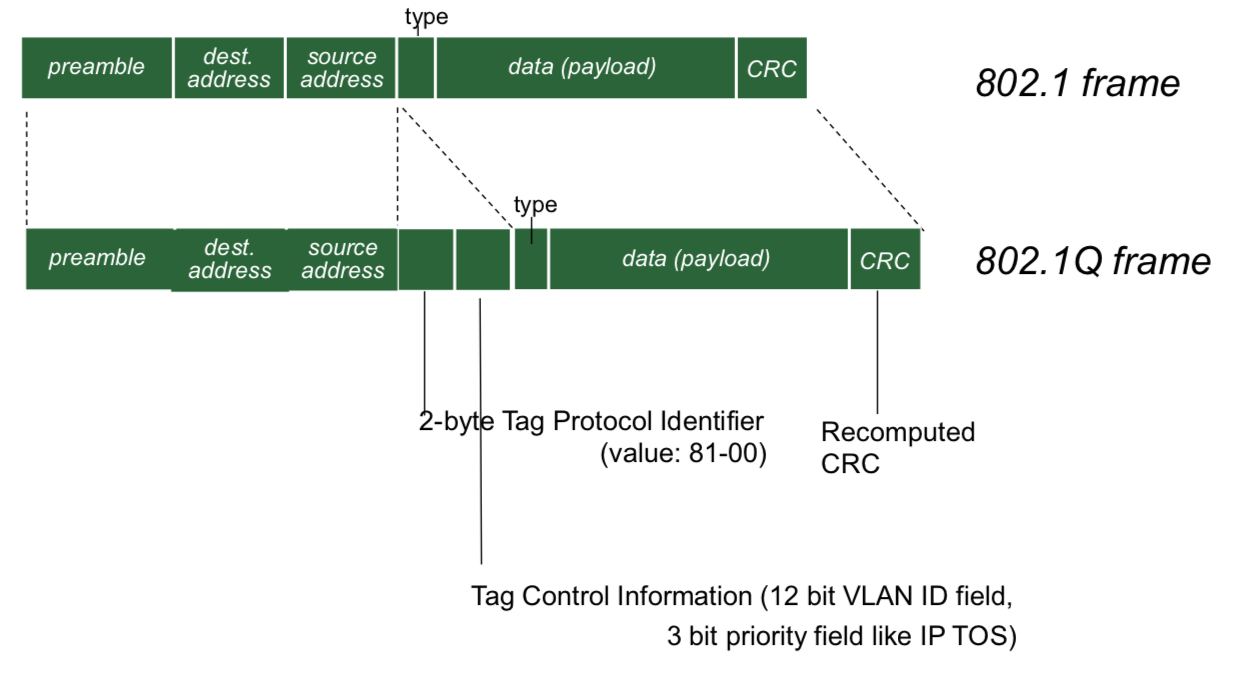
\includegraphics[width=\linewidth]{802q}
	\centering
	\caption{802.1Q VLAN frame format}
\end{figure}
	
	\section{Chapter 7}
	% !TeX spellcheck = en_US
% !TeX root = notes.tex
\subsection{Wireless}
\begin{figure}[H]
	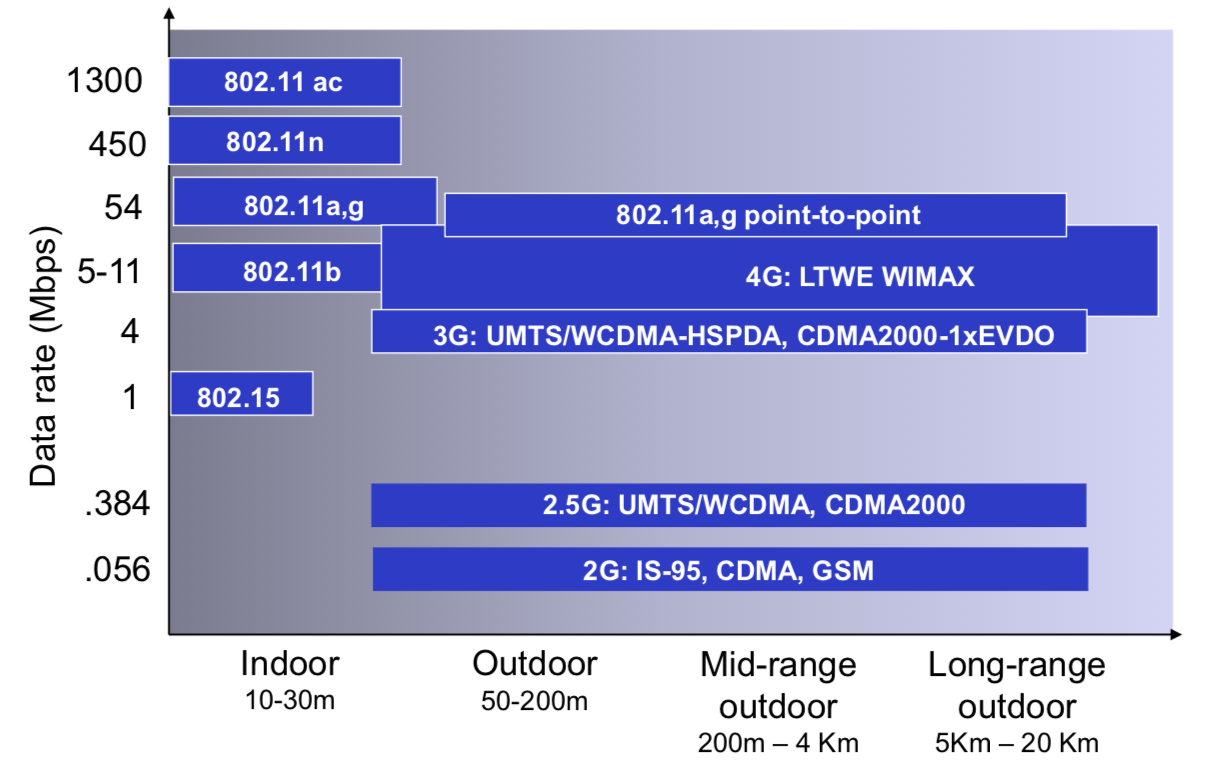
\includegraphics[width=\linewidth]{wifi}
	\centering
	\caption{Characteristics of selected wireless links}
\end{figure}
\subsubsection{Infrastructure mode}
\begin{itemize}
	\item base station connects mobiles into wired network
	\item handoff: mobile changes base station providing connection into wired network
\end{itemize}
\subsubsection{Ad Hoc mode}
\begin{itemize}
	\item no base stations
	\item nodes can only transmit to other nodes within link coverage
	\item nodes organize themselves into a network: route among themselves
\end{itemize}
\begin{table}[H]
	\centering
	\caption{Wireless Network Taxonomy}
	\begin{tabular}{p{2.5cm}|p{3cm}p{3cm}}
		\toprule
		&\textbf{single hop} & \textbf{multiple hops}\\
		\midrule
		\textbf{infrastructure (e.g. APs)} & host connects to base station (WiFi, WiMAX, cellular) which connects to larger Internet & host may have to relay through several wireless nodes to connect to larger Internet: mesh net\\
		\midrule
		\textbf{no infrastructure} & no base station, no connection to larger Internet (Bluetooth, ad hoc nets) & no base station, no connection to larger Internet. May have to relay to reach another given wireless node. MANET, VANET\\
		\bottomrule
	\end{tabular}
\end{table}
\subsubsection{Wireless Link Characteristics}
\textbf{important} difference from wired link...
\begin{description}
	\item[decreased signal strength:] radio signal attenuates as it propagates through matter (path loss)
	\item[interference from other sources:] standardized wireless network frequencies (e.g. 2.4GHz) shared by other devices (e.g. phone); devices (motors) interfere as well
	\item[multipath propagation:] radio signal reflects off objects ground, arriving ad destination at slightly different times
\end{description}
...make communication across (even a point to point) wireless link much more ``difficult''\\
SNR: signal-to-noise ratio. Larger SNR -- easier to extract signal from noise (a ``good thing'')\\
\textbf{SNR versus BER tradeoffs}
\begin{description}
	\item[given physical layer:] increase power $\rightarrow$ increase SNR $\rightarrow$ decrease BER
	\item[given SNR:] choose physical layer that meets BER requirement, giving highest throughput (SNR may change with mobility: dynamically adapt physical layer (modulation technique, rate)
\end{description}
\subsubsection{Code Division Multiple Access (CDMA)}
\begin{itemize}
	\item unique ``code'' assigned to each user; i.e. code set partitioning
	\begin{itemize}
		\item all users share same frequency, but each user has own ``chipping'' sequence (i.e. code) to encode data
		\item allows multiple users to ``coexist'' and transmit simultaneously with minimal interference (if codes are ``orthogonal'')
	\end{itemize}
	\item \textbf{encoded signal} = (original data) $\times$ (chipping sequence)
	\item \textbf{decoding:} inner-product of encoded signal and chipping sequence
\end{itemize}

\subsection{IEEE 802.11 Wireless LAN}
\textbf{802.11b}
\begin{itemize}
	\item 2.4 - 5 GHz unlicensed spectrum
	\item up to 11 Mbps
	\item direct sequence spread spectrum (DSSS) in physical layer (all hosts use same chipping code)
\end{itemize}
\textbf{802.11a}
\begin{itemize}
	\item 5 - 6 GHz range
	\item up to 54 Mbps
\end{itemize}
\textbf{802.11g}
\begin{itemize}
	\item 2.4 - 5 GHz
	\item up to 54 Mbps
\end{itemize}
\textbf{802.11n:} multiple antennae
\begin{itemize}
	\item 2.4 - 5 GHz range
	\item up to 200 Mbps
\end{itemize}
All use CSMA/CA for multiple access. All have base-station and ad-hoc network versions
\subsubsection{802.11 LAN architecture}
\begin{itemize}
	\item wireless host communicates with base station (base station = access point (AP))
	\item \textbf{Basic Service Set (BSS)} (aka ``cell'') in infrastructure mode contains:
	\begin{itemize}
		\item wireless hosts
		\item access point (AP): base station
		\item ad hoc mode: hosts only
	\end{itemize}
\end{itemize}
\subsubsection{Channels, association}
\begin{itemize}
	\item 802.11b: 2.4GHz - 2.485GHz spectrum divided into 11 channels at different frequencies
	\begin{itemize}
		\item AP admin chooses frequency for AP
		\item interference possible: channel can be same as that chosen by neighboring AP
	\end{itemize}
	\item host: must \textbf{associate} with an AP
	\begin{itemize}
		\item scans channels, listening for \textit{beacon frames} containing AP's name (SSID) and MAC address
		\item selects AP to associate with
		\item may perform authentication
		\item will typically run DHCP to get IP address in AP's subnet
	\end{itemize}
\end{itemize}
\begin{leftbar}
	802.11 has no collision detection
\end{leftbar}
\subsubsection{IEEE 802.11 MAC Protocol: CSMA/CA}
\textbf{802.11 sender}
\begin{enumerate}
	\item if sense channel idle for \textbf{DIFS} then transmit entire frame (no CD)
	\item if sense channel busy then:
	\begin{enumerate}
		\item start random backoff time
		\item timer counts down while channel idle
		\item transmit when timer expires
		\item if no ACK, increase random backoff interval, repeat 2
	\end{enumerate}
\end{enumerate}
\textbf{802.11 receiver}
If frame received OK $\rightarrow$ return ACK after \textbf{SIFS} (ACK needed due to hidden terminal problem)
\begin{figure}[H]
	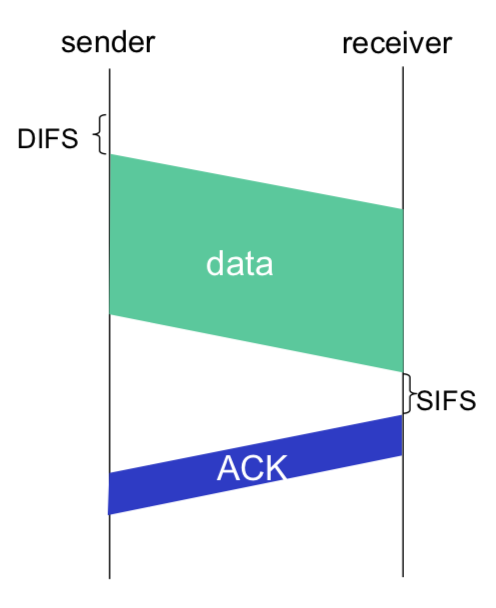
\includegraphics[width=0.5\linewidth]{proto}
	\centering
	\caption{802.11 CSMA/CA}
\end{figure}
\textbf{Avoiding Collisions}
\begin{itemize}
	\item sender first transmits \textit{small} request-to-send (RTS) packets to BS using CSMA (RTSs may still collide with each other (but they're short)
	\item BS broadcasts clear-to-send (CTS) in response to RTS
	\item CTS heard by all nodes (sender transmits data frame, other stations defer transmissions
\end{itemize}
\end{multicols*}
\subsubsection{802.11 frame: addressing}
\begin{table}[H]
	\centering
	\caption{802.11 frame}
	\begin{tabular}{cccccp{1.8cm}ccc}
		2&2&6&6&6&2&6&0-2312&4\\
		\midrule
		frame control & duration & address 1 & address 2 & address 3 & sequence control & address 4 & payload & CRC
	\end{tabular}
\end{table}
\begin{table}[H]
	\centering
	\caption{Frame Control Break Down}
	\begin{tabular}{p{1.5cm}cccp{0.8cm}cccccc}
		2&2&4&1&1&1&1&1&1&1&1\\
		\midrule
		Protocol version & Type & Subtype & To AP & From AP & More frag & Retry & Power mgt & More data & WEP & Rsvd
	\end{tabular}
\end{table}
\begin{multicols*}{2}
\begin{description}
	\item[Address 1:] MAC address of wireless host or AP to receive this frame
	\item[Address 2:] MAC address of wireless host or AP transmitting this frame
	\item[Address 3:] MAC address of router interface to which AP is attached
	\item[Address 4:] used only in ad hoc mode
\end{description}
\subsection{802.11 Power Management}
\begin{itemize}
	\item node-to-AP: Sleeping till next frame (AP knows not to transmit frames to this node, node wakes up before next beacon frame)
	\item beacon frame: contains list of mobiles with AP-to-mobile frames waiting to be sent (node will stay awake if AP-to-mobile frames to be sent; otherwise sleep again until next beacon frame
\end{itemize}
\subsection{802.15: Personal Area Network}
\begin{itemize}
	\item less than 10m diameter
	\item replacement for cables (mouse, keyboard, headphones)
	\item ad hoc: no infrastructure
	\item master/slaves: (slaves request permission to send (to master), master grants requests)
	\item 802.15: evolved from Bluetooth specification (2.4 - 2.5 GHz radio band, up to 721 kbps)
\end{itemize}
\begin{figure}[H]
	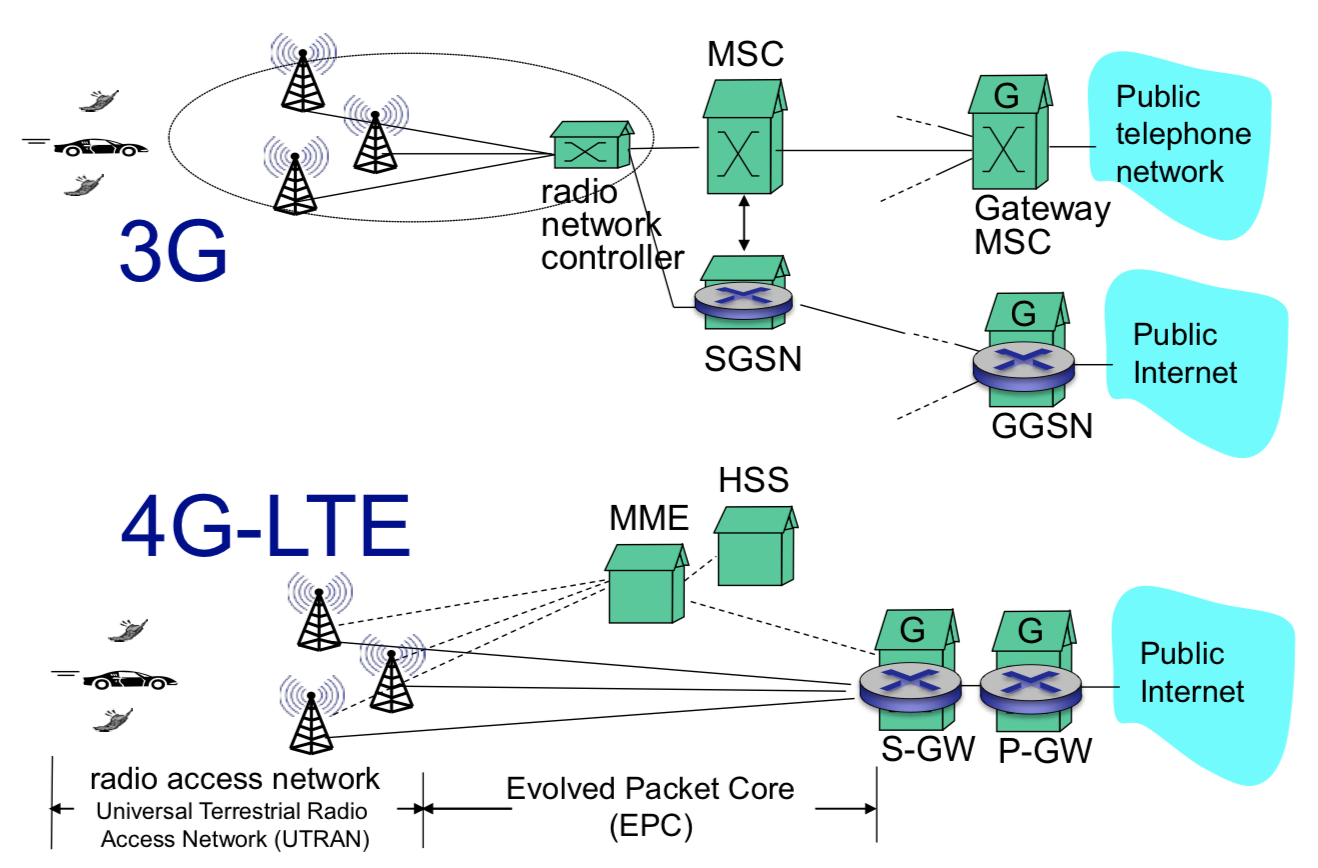
\includegraphics[width=\linewidth]{4G}
	\centering
	\caption{3G vs 4G LTE}
\end{figure}
	
	\section{Chapter 8}
	% !TeX spellcheck = en_US
% !TeX root = notes.tex
\subsection{What is network security}
\begin{description}
	\item[confidentiality:] only sender, intended receiver should ``understand'' message contents (sender encrypts message, receiver decrypts message)
	\item[authentication:] sender, receiver want to conform identity of each other
	\item[message integrity:] sender, receiver want to ensure message not altered (in transit, or afterwards) without detection
	\item[access and availability:] services must be accessible and available to users
\end{description}
What can a ``bad guy'' do?
\begin{itemize}
	\item \textbf{eavesdrop:} intercept messages
	\item actively \textbf{insert} messages into connection
	\item \textbf{impersonation:} can fake (spoof) source address in packet (or any field in packet)
	\item \textbf{hijacking:} ``take over'' ongoing connection by removing sender or receiver, inserting himself in place
	\item \textbf{denial of service:} prevent service from being used by other (e.g. by overloading resources)
\end{itemize}
\subsubsection{Breaking an encryption scheme}
\begin{description}
	\item[cipher-text only attack:] Trudy has ciphertext she can analyze
	\item[two approaches:] brute force: search through all keys. Statistical analysis
	\item[known-plaintext attack:] Trudy has plaintext corresponding to ciphertext (e.g. in monoalphabetic cipher, Trudy determines pairings for a,l,i,c,e,b,o)
	\item[chosen-plaintext attack:] Trudy can get ciphertext for chosen plaintext
\end{description}

\subsection{Symmetric Key Cryptography}
Bob and Alice share same (symmetric) key, e.g. key is knowing substitution pattern in mono alphabetic substitution cipher
\subsubsection{Substitution Cipher}
substituting one thing for another. Monoalphabetic cipher: substitute one letter for another.\\\\
Make it more sophisticated by adding cycling pattern. For $n$ substitution ciphers: $M_1, M_2, \ldots, M_n$. Cycling pattern: $n=4\quad M_1,M_3,M_4,M_3,M_2$. Example: dog, d from $M_1$, o from $M_3$, g from $M_4$. Need to send $n$ substitution ciphers and cyclic pattern
\subsubsection{DES: Date Encryption Standard}
\begin{itemize}
	\item US encryption standard [NIST 1993]
	\item 56-bit symmetric key, 64-bit plaintext input
	\item block cipher with cipher block chaining
	\item 56-bit-key-encrypted phrase decrypted (brute force) in less than a day
	\item no known good analytic attack
	\item making DES more secure: \textbf{3DES}, encrypt 3 times with 3 different keys
\end{itemize}
\subsubsection{AES: Advanced Encryption Standard}
\begin{itemize}
	\item symmetric-key NIST standard, replaced DES (Nov 2001)
	\item processes data in 128 bit blocks
	\item 128, 192, or 256 bit keys
	\item brute force decryption (try each key) taking 1 sec on DES, takes 149 trillion years for AES
\end{itemize}

\subsection{Public Key Cryptography}
\begin{itemize}
	\item radically different approach (Diffie-Hellman76, RSA78)
	\item sender, receiver do not share secret key
	\item public encryption key known to all
	\item private decryption key known only to receiver
\end{itemize}
\begin{note}{Why is RSA secure?}
	\begin{itemize}
		\item suppose you know Bob's public key $(n,e)$. How hard is it to determine $d$?
		\item essentially need to find factors of $n$ without knowing the two factors $p$ and $q$ (factoring a big number is hard)
	\end{itemize}
\end{note}
\textbf{RSA in practice}
\begin{itemize}
	\item exponentiation in RSA is computationally intesive
	\item DES is at least 100 times faster than RSA
	\item use public key crypto to establish secure connection, then establish second key -- symmetric session key -- for encrypting data
\end{itemize}

\subsection{Authentication}
Can use nonce (a once-in-a-lifetime value) to encrypt the password. This is still open to a man-in-the-middle attack, and is undetectable.

\subsection{Digital Signatures}
\textbf{Cryptographic technique analogous to hand-written signatures}
\begin{itemize}
	\item sender digitally signs document, establishing he is document owner/creator
	\item verifiable, nonforgeable: recipient can prove to someone that sender, and no one else (including receiver), must have signed document
	\item encrypt the document with private key, the document can only be decrypted with public key
\end{itemize}

\subsection{Hashing}
\begin{itemize}
	\item produces a fixed length message size
	\item many-to-1
	\item given $x$ computationally infeasible to find $m$ such that $x=H(m)$
\end{itemize}
\textit{Internet checksum is poor hash algorithm, easy to find message with same hash}
\begin{note}{Signed Message Hash}
	Because Public Key Cryptography is computationally heavy for a large message, hash the message then sign the hash. Then the receiver can hash the message and apply the public key to see if they match
\end{note}
\subsubsection{Hash Algorithms}
\begin{itemize}
	\item \textbf{MD5 hash function widely used (RFC 1321)}
	\begin{itemize}
		\item computes 128-bit message digest in 4-step process
		\item arbitrary 128-bit string $x$, appears difficult to construct message $m$ whose MD5 hash is equal to $x$
	\end{itemize}
	\item \textbf{SHA-1 is also used}
	\begin{itemize}
		\item US standard [NIST, FIPS PUB 180-1]
	\end{itemize}
\end{itemize}

\subsection{Certification Authorities}
\begin{itemize}
	\item \textbf{certification authority (CA):} binds public key to particular entity, $E$
	\item $E$ (person, router) registers its public key with CA.
	\begin{itemize}
		\item $E$ provides ``proof of identity'' to CA
		\item CA creates certificate binding $E$ to its public key
		\item certificate containing $E$'s public key digitally signed by CA -- CA says ``this is $E$'s public key''
	\end{itemize}
\end{itemize}

\subsection{SSL: Secure Sockets Layer}
\begin{itemize}
	\item widely deployed security protocol (supported by almost all browser, web servers), (https, billions of \$/year over SSL)
	\item variation -TLS, RFC 2246
	\item provides:
	\begin{itemize}
		\item confidentiality
		\item integrity
		\item authentication
	\end{itemize}
	\item available to all TCP applications (secure socket interface)
	\item SSL provides application programming interface (API) to applications
	\item SSL is considered an application layer protocol on top of TCP, but used by programmers like a transport service
\end{itemize}
\begin{note}{Toy SSL: simple secure channel}
	\begin{enumerate}
		\item \textbf{handshake:} Alice and Bob use their certificates, private keys to authenticate each other and exchange shared secret
		\item \textbf{key derivation:} Alice and Bob use shared secret to derive set of keys
		\item \textbf{data transfer:} data to be transferred is broken up into series of records
		\item \textbf{connection closure:} special messages to securely close connection
	\end{enumerate}
\end{note}
\subsubsection{SSL cipher suite}
\begin{itemize}
	\item cipher suite (public-key algorithm, symmetric encryption algorithm, MAC algorithm)
	\item SSL supports several cipher suites
	\item negotiation: client, server agree on cipher suite (client offers choice, server picks one)
\end{itemize}
\begin{note}{Common SSL Algorithms}
	\textbf{common SSL symmetric ciphers}
	\begin{itemize}
		\item DES -- Data Encryption Standard: block
		\item 3DES -- Triple strength: block
		\item RC2 -- Rivest Cipher 2: block
		\item RC4 -- Rivest Cipher 4: stream
	\end{itemize}
	\textbf{SSL Public key encryption}
	\begin{itemize}
		\item RSA
	\end{itemize}
\end{note}
\begin{table}[H]
	\centering
	\caption{SSL record format}
	\begin{tabular}{ccccc}
		1 byte & 2 bytes & 3 bytes &&\\
		\midrule
		content type & SSL version & length & data & MAC
	\end{tabular}
\end{table}
\textit{data and MAC encrypted (symmetric algorithm)}

\subsection{Network-layer Security}
\subsubsection{What is network-layer confidentiality}
\begin{itemize}
	\item sending entity encrypts datagram payload, payload could be: TCP or UDP segment, ICMP message, OSPF message...
	\item all data sent from one entity to other would be hidden: web pages, e-mail, P2P file transfers, TCP SYN packets
	\item \textbf{``blanket coverage''}
\end{itemize}
\subsubsection{Virtual Private Networks (VPNs)}
VPN: institution's inter-office traffic is sent over public Internet instead
\begin{itemize}
	\item encrypted before entering public Internet
	\item logically separate from other traffic
\end{itemize}
\subsubsection{IPsec services}
\begin{itemize}
	\item data integrity
	\item origin authentication
	\item replay attack prevention
	\item confidentiality
	\item two protocols providing different service models:
	\begin{itemize}
		\item Authentication Header (AH) protocol $\rightarrow$ provides source authentication and data integrity but not confidentiality
		\item Encapsulation Security Protocol (ESP) $\rightarrow$ provides source authentication, data integrity, and confidentiality. More widely used than AH
	\end{itemize}
	\item two modes:
	\begin{itemize}
		\item host mode: host computers encrypt and decrypt
		\item tunneling mode: edge routers IPsec-aware
	\end{itemize}
\end{itemize}
\begin{figure}[H]
	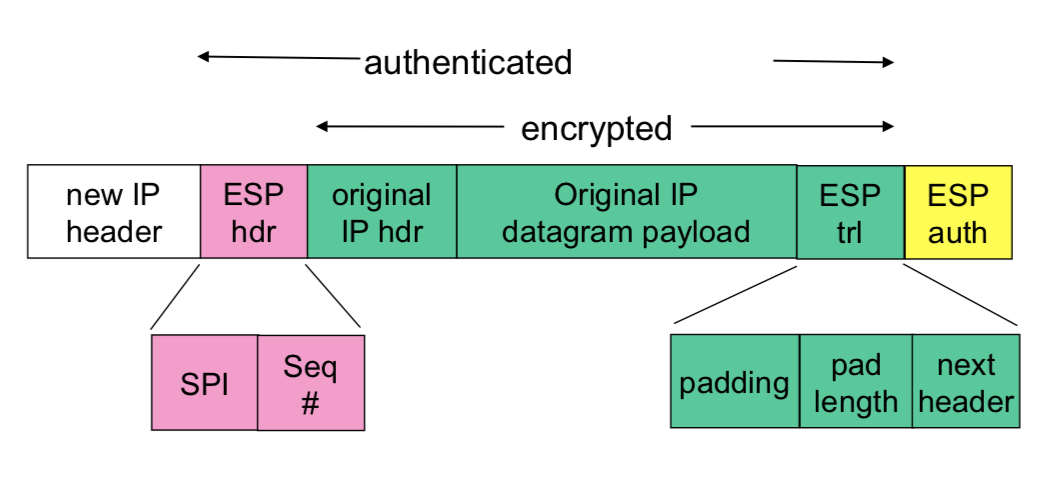
\includegraphics[width=\linewidth]{ipsec}
	\centering
	\caption{IPsec datagram (tunnel, ESP)}
\end{figure}
\begin{itemize}
	\item IKE message exchange for algorithms, secret keys, SPI numbers
\end{itemize}

\subsection{Firewalls}
\begin{description}
	\item[prevent DoS attacks:] SYN flooding, attacker establishes many bogus TCP connections, no resources left for ``real'' connections
	\item[prevent illegal modification/access of internal data:] e.g. attack replaces CIA's homepage with something else
	\item[allow only authorized access to inside network:] set of authenticated users/hosts
	\item[three types of firewalls:] stateless packet filters, stateful packet filters, application gateways
\end{description}
\subsubsection{Limitations of firewalls, gateways}
\begin{itemize}
	\item \textbf{IP spoofing:} router can't know if data ``really'' comes from claimed source
	\item if multiple applications need special treatment, each has own application gateway
	\item client software must know how to contact gateway (e.g. must set IP address of proxy in Web browser)
	\item filters often use all or nothing policy for UDP
	\item \textbf{tradeoff:} degree of communication with outside world, level of security
	\item many highly protected sites still suffer from attacks
\end{itemize}
\subsubsection{Intrusion detection systems}
\begin{itemize}
	\item packet filtering:
	\begin{itemize}
		\item operates on TCP/IP headers only
		\item no correlation check among sessions
	\end{itemize}
	\item \textbf{IDS:} Intrusion detection system
	\begin{description}
		\item[deep packet inspection:] look at packet contents (e.g. check character strings in packet against database of known virus, attack strings
		)
		\item[examine correlation] among multiple packets (port scanning, network mapping, DoS attack)
	\end{description}
\end{itemize}
	
	\section{Chapter 9}
	% !TeX spellcheck = en_US
% !TeX root = notes.tex
\subsection{Multimedia}
\subsubsection{Audio}
\begin{itemize}
	\item Analog audio signal sampled at constant rate (telephone: 8000 samples/sec, CD music: 44,100 samples/sec)
	\item quantized, i.e. rounded (8 bits for 256 values)
	\item Example rates (CD: 1.411 Mbps, MP3: 96,128,160 kbps, Internet Telephony: 5.3 kpbs)
\end{itemize}
\subsubsection{Video}
\begin{itemize}
	\item MPEG 1 (CD-ROM) 1.5 Mbps
	\item MPEG 2 (DVD) 3-6 Mbps
	\item MPEG 4 (often used in Internet) <1 Mbps
\end{itemize}
\subsubsection{3 Application Types}
\begin{itemize}
	\item\textbf{Streaming, stored} audio, video
	\begin{description}
		\item[streaming:] can begin playout before downloading entire file
		\item[stored (at server):] can transmit faster than audio/video will be rendered (implies storing/buffering at client)
	\end{description}
	\item\textbf{conversational} voice/video over IP (interactive nature of human-to-human conversation limits delay tolerance
	\item\textbf{streaming live} audio, video
	\item Once playout begins, playback must match original timing (network delays are variable)
	\begin{itemize}
		\item\textbf{Client-side buffer} to match playout requirements
	\end{itemize}
	\item RTP [RFC 2326] multimedia payload types
\end{itemize}

\subsection{Voice-over-IP (VoIP)}
\begin{itemize}
	\item\textbf{VoIP end-end-delay requirement:} needed to maintain ``conversational'' aspect (< 150msec: good, > 400msec bad)
	\item\textbf{session initialization:} how does callee advertise IP address, port number, encoding algorithms?
	\item\textbf{value-added services:} call forwarding, screening, recording
	\item\textbf{emergency services:} 911
	\item\textbf{network loss:} IP datagram lost due to network congestion (router buffer overflow)
	\item\textbf{delay loss:} IP datagram arrives too late for playout at receiver
	\item\textbf{loss tolerance:} depending on voice encoding, loss concealment, packet loss rates between 1\% and 10\% can be tolerated
\end{itemize}
\subsubsection{Adaptive playout delay}
\begin{itemize}
	\item estimate network delay, adjust playout delay at beginning of each talk spurt
	\item silent periods compressed and elongated
\end{itemize}
$$ d_i = (1-\alpha)d_{i-1}+\alpha(r_i-t_i) $$
\begin{description}
	\item[$d_i$:] delay estimate after ith packet
	\item[$\alpha$:] small constant e.g. 0.1
	\item[$r_i$:] time received
	\item[$t_i$:] time sent (timestamp)
\end{description}
\subsubsection{Recovery from packet loss}
\textbf{simple FEC (Forward Error Correction)}
\begin{itemize}
	\item for every group of $n$ chunks, create redundant chunk by exclusive OR-ing $n$ original chunks
	\item send $n+1$ chunks, increasing bandwidth by factor $\frac{1}{n}$
	\item can reconstruct original $n$ chunks if at most one lost chunk from $n+1$ chunks, with playout delay
\end{itemize}
%\subsubsection{Skype}
%\begin{leftbar}
%	Proprietary application-layer protocol (inferred via reverse engineering) $\rightarrow$ encrypted messages
%\end{leftbar}
%\begin{figure}[H]
%	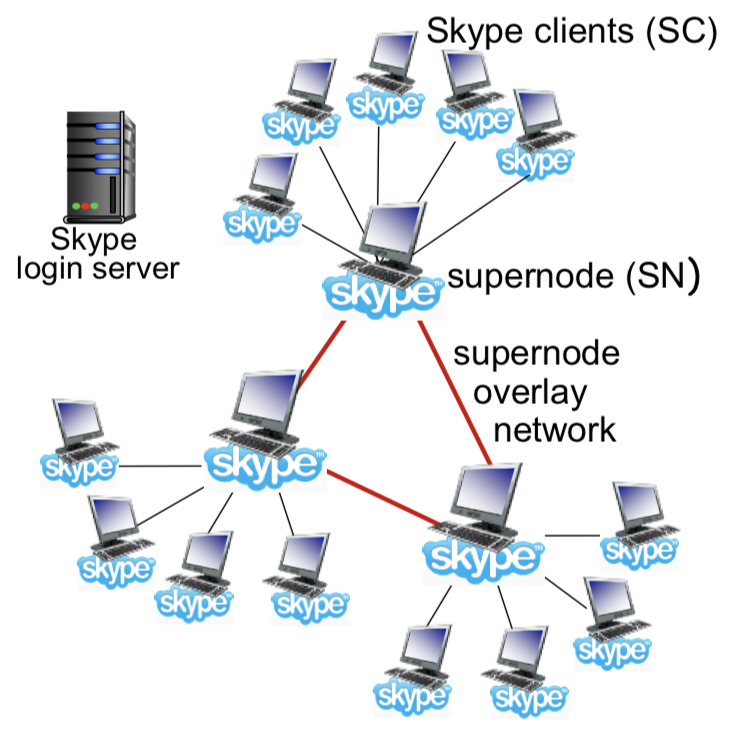
\includegraphics[width=\linewidth]{skype}
%	\centering
%	\caption{Skype Network Layout}
%\end{figure}
%P2P components:
%\begin{description}
%	\item[clients:] Skype peers connect directly to each other for VoIP call
%	\item[super nodes (SN):] Skype peers with special functions
%	\item[overlay network:] among SNs to locate SCs
%	\item[login server]
%\end{description}

\subsection{Real-Time Protocol (RTP)}
\begin{itemize}
	\item RTP specifies packet structure for packets carrying audio, video data
	\item RFC 3550
	\item RTP packet provides
	\begin{itemize}
		\item payload type identification
		\item packet sequence numbering
		\item time stamping
	\end{itemize}
	\item RTP runs in end systems
	\item RTP packets encapsulated in UDP segments
	\item interoperability: if two VoIP applications run RTP, they may be able to work together
\end{itemize}
\subsubsection{RTP runs on top of UDP}
RTP libraries provide transport-layer interface that extends UDP:
\begin{itemize}
	\item port numbers, IP addresses
	\item payload type identification
	\item packey sequence numbering
	\item time-stamping
\end{itemize}
\subsubsection{RTP and QoS}
\begin{itemize}
	\item RTP does \textbf{not} provide any mechanism to ensure timely data delivery or other QoS guarantees
	\item RTP encapsulation only seen at end systems (not by intermediate routers)
	\subitem routers provide best-effort service, making no special effort to ensure that RTP packets arrive at destination in timely matter
\end{itemize}

\subsection{Real-Time Control Protocol (RTCP)}
\begin{itemize}
	\item works in conjuncation with RTP
	\item each participant in RTP session periodically sends RTCP control packets to all other participants
	\item each RTCP packet contains sender and/or receiver reports
	\subitem report statistics useful to application: \# packets sent, \# packets lost, interarrival jitter
	\item feedback used to control performance
	\subitem sender may modify its transmissions based on feedback
\end{itemize}
\subsubsection{RTCP: packet types}
\begin{description}
	\item[receiver report packets:] fraction of packets lost, last sequence number, average interarrival jitter
	\item[sender report packets:] SSRC of RTP stream, current time, number of packets sent, number of bytes sent
	\item[source description packets:] email address of sender, sender's name, SSRC of associated RTP stream. Provide mapping between the SSRC and the user/host name
\end{description}

\subsection{SIP: Session Initiation Protocol}
\textbf{long-term vision:}
\begin{itemize}
	\item all telephone calls, video conference calls take place over Internet
	\item people identified by names or e-mail addresses, rather than by phone numbers
	\item can reach callee (if callee so desires), no matter where callee roams, no matter what IP device callee is currently using
\end{itemize}
\subsubsection{SIP services}
\begin{itemize}
	\item SIP provides mechanisms for call setup:
	\begin{itemize}
		\item for caller to let callee know she wants to establish a call
		\item so caller, callee can agree on media type, encoding
		\item to end call
	\end{itemize}
	\item determine current IP address of callee: maps mnemonic identifier to current IP address
	\item call management:
	\begin{itemize}
		\item add new media streams during call
		\item change encoding during call
		\item invite others
		\item transfer, hold calls
	\end{itemize}
\end{itemize}
\textit{SIP default port 506}\\
\textbf{SIP registrar}\\
Function of SIP server (registrar). When Bob starts SIP client, client sends SIP REGISTER message to Bob's registrar server\\
\textbf{SIP proxy}\\
Function of SIP server (proxy). Alice sends invite message to her proxy, proxy responsible for routing SIP messages to callee possibly through multiple proxies. Bob sends response back through same set of SIP proxies, proxy returns Bob's SIP response message to Alice. SIP proxy analogous to local DNS server plus TCP setup

\begin{note}{Comparison with H.323}
	\begin{itemize}
		\item Another signaling protocol for real-time, interactive multimedia
		\item Complete, vertically integrated suite of protocols for multimedia conferencing; signaling, registration, admission control, transport, codecs
		\item SIP is a single component. Works with RTP, but does not mandate it. Can be combined with other protocols, services
		\item SIP uses KISS principle
	\end{itemize}
\end{note}
	
	\section{Day in the life of a web request}
	\subsection{Connecting to the Internet}
	\begin{itemize}
		\item connecting laptop needs to get its own IP address, addr of first-hop router, addr of DNS server: use \textbf{DHCP}
		\item DHCP request \textbf{encapsulated} in \textbf{UDP}, encapsulated in \textbf{IP}, encapsulated in \textbf{802.3} Ethernet
		\item Ethernet frame \textbf{broadcast} (dest: FFFFFFFFFFFF) on LAN received at router running \textbf{DHCP} server
		\item Ethernet \textbf{demuxed} to IP demuxed, UDP demuxed to DHCP
		\item DHCP server formulates \textbf{DHCP ACK} containing client's IP address, IP address of first-hop router for client, name and IP address of DNS server
		\item encapsulate at DHCP server, frame forwarded (\textbf{switch learning}) through LAN, demultiplexing at client
		\item DHCP client receives DHCP ACK reply
	\end{itemize}
	\textit{Client now has IP address, knows name and addr of DNS server, IP address of its first-hop router}
	\subsubsection{ARP (before DNS, before HTTP)}
	\begin{itemize}
		\item before sending \textbf{HTTP} request, need IP address of www.google.com: \textbf{DNS}
		\item DNS query created, encapsulated in UDP, encapsulated in IP, encapsulated in Ethernet. To send frame to router, need MAC address of router interface: \textbf{ARP}
		\item\textbf{ARP query} broadcast, received by router, which replies with \textbf{ARP reply} giving MAC address of router interface
		\item client now knows MAC address of first hop router, so can now send frame containing DNS query
	\end{itemize}
	\subsubsection{using DNS}
	\begin{itemize}
		\item IP datagram containing DNS query forwarded via LAN switch from client to $1^{st}$ hop router
		\item IP datagram forwarded from campus network into Comcast network, routed (tables created by \textbf{RIP, OSPF, IS-IS} and/or \textbf{BGP} routing protocols) to DNS server
		\item demuxed to DNS server
		\item DNS server replies to client with IP address of www.google.com
	\end{itemize}
	\subsubsection{TCP connection carrying HTTP}
	\begin{itemize}
		\item to send HTTP request, client first opens \textbf{TCP socket} to web server
		\item TCP \textbf{SYN segment} (step 1 in 3-way handshake) inter-domain routed to web server
		\item web server responds with \textbf{TCP SYNACK} (step 2 in 3-way handshake)
		\item TCP \textbf{connection established}
	\end{itemize}
	\subsubsection{HTTP request/reply}
	\begin{itemize}
		\item \textbf{HTTP request} sent into TCP socket
		\item IP datagram containing HTTP request routed to www.google.com
		\item web server responds with \textbf{HTTP reply} (containing web page)
		\item IP datagram containing HTTP reply routed back to client
	\end{itemize}
	
\end{multicols*}	
	
	\newpage
	\section{Packet Format}
	% !TeX spellcheck = en_US
% !TeX root = notes.tex
\subsection{Application Layer}
% HTTP request, reply
\subsubsection{Request Message}
\begin{figure}[H]
	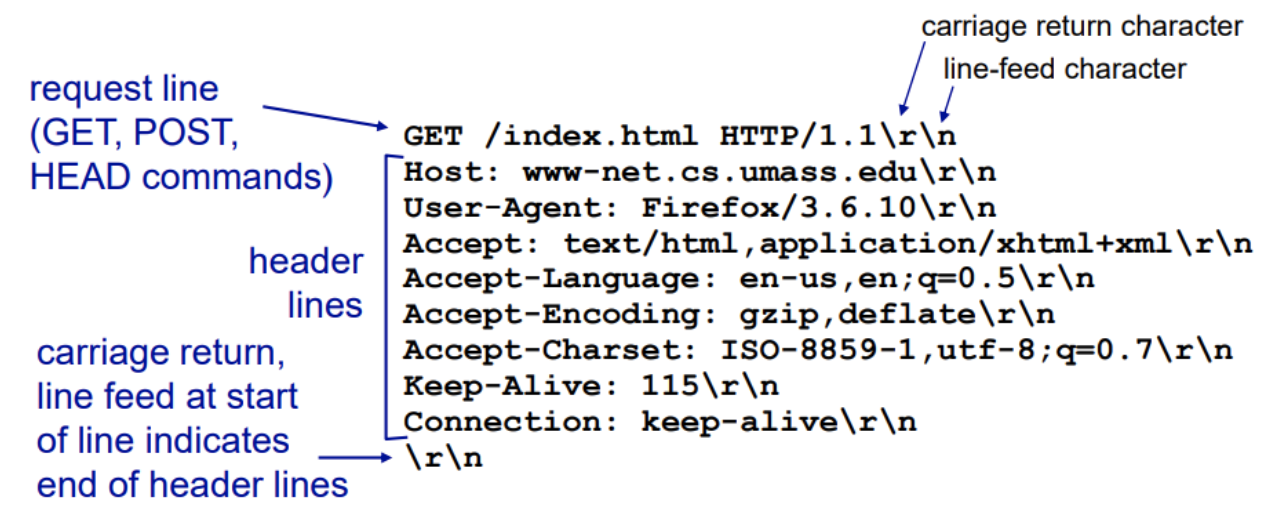
\includegraphics[width=\linewidth]{request}
	\centering
	\caption{HTTP Request Message}
\end{figure}
\subsubsection{Response Message}
\begin{figure}[H]
	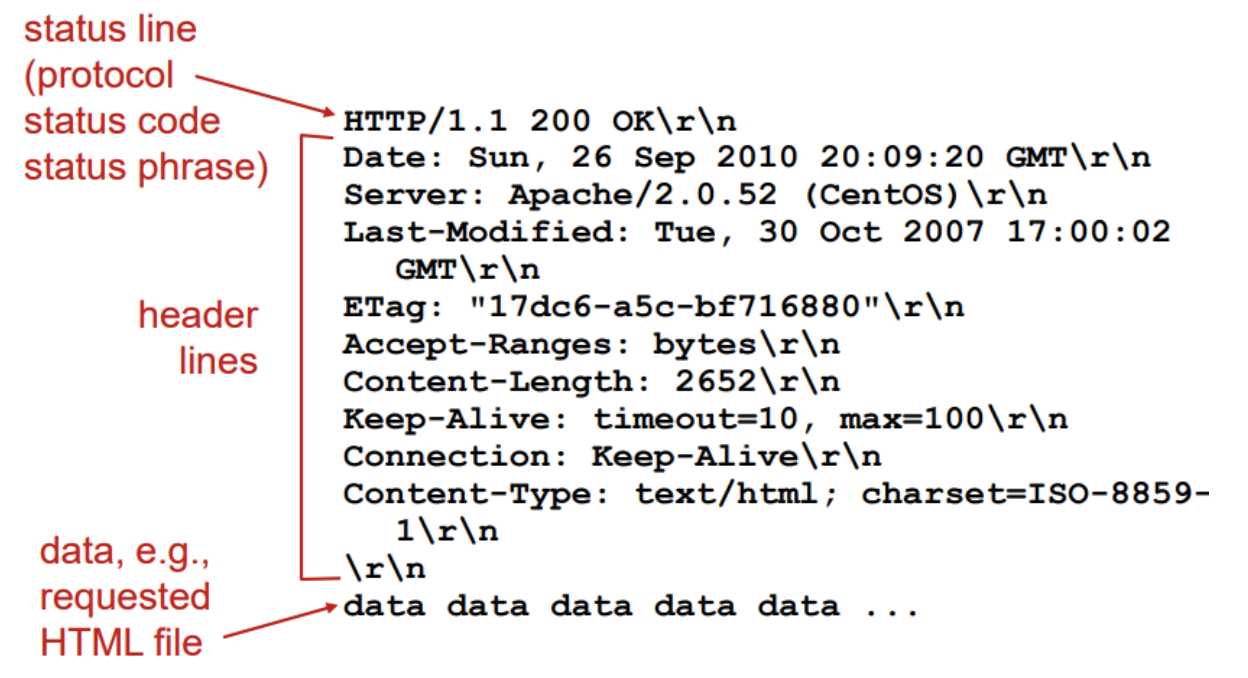
\includegraphics[width=\linewidth]{response}
	\centering
	\caption{HTTP Response Message}
\end{figure}

\subsection{Presentation}
\textbf{ISO/OSI Reference:} Allow applications to interpret meaning of data, e.g. encryption, compression, machine-specific conventions
\subsection{Session}
\textbf{ISO/OSI Reference:} Synchronization, check-pointing, recovery of data exchange

\subsection{Transport Layer}
% TCP, UDP
\subsubsection{UDP}
\begin{table}[H]
	\centering
	\caption{UDP Breakdown}
	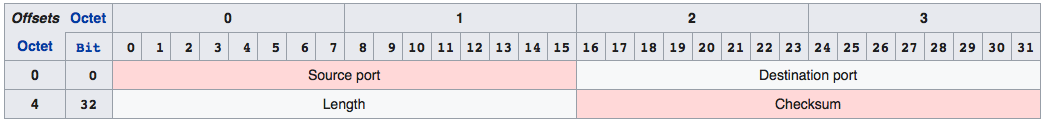
\includegraphics[width=\linewidth]{udp}
\end{table}
\begin{description}
	\item[Source Port:] Sender's port number
	\item[Destination Port:] Receiver's port number
	\item[Length:] Length of UDP header and data in bytes. Min is 8, max is 65,535 bytes
	\item[Checksum:] Optional for IPv4
\end{description}
\subsubsection{TCP}
\begin{table}[H]
	\centering
	\caption{TCP Breakdown}
	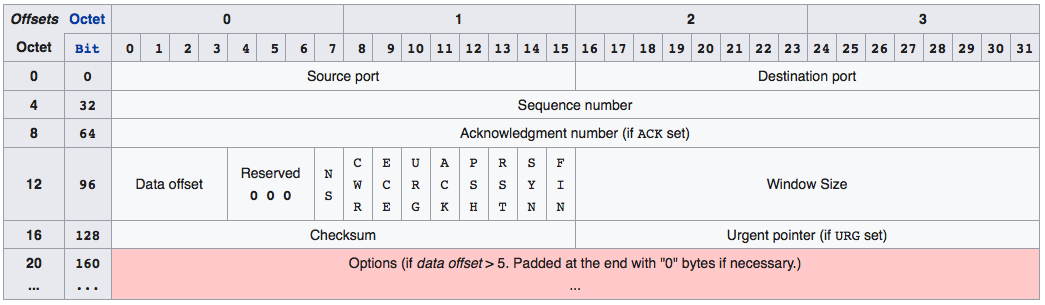
\includegraphics[width=\linewidth]{tcp}
\end{table}
\begin{description}
	\item[Source Port:] Sending Port
	\item[Destination Port:] Receiving Port
	\item[Sequence Number:] If the \texttt{SYN} flag is set (1), then this is the initial sequence number. The sequence number of the actual first data byte and the acknowledged number in the corresponding ACK are then this sequence number plus 1
	\subitem If the \texttt{SYN} flag is clear (0), then this is the accumulated sequence number of the first data byte of this segment for the current session
	\item[Acknowledgment number:] If the \texttt{ACK} flag is set then the value of this field is the next sequence number that the sender of the ACK is expecting. This acknowledges receipt of all prior bytes (if any). The first \texttt{ACK} sent by each end acknowledges the other end's initial sequence number itself, but no data
	\item[Data offset:] Size of TCP header in 32-bit words. Min 5, Max 15 words (max of 60 bytes $\rightarrow$ 40 byte options)
	\item[Flags:]
	\begin{description}
		\item[NS:] ECN-nonce concealment
		\item[CWR:] Congestion Window Reduction
		\item[ECE:] ECN-Echo
		\item[URG:] Urgent pointer field is significant
		\item[ACK:] Acknowledgment field is significant
		\item[PSH:] Push function
		\item[RST:] Reset the connection
		\item[SYN:] Synchronize sequence numbers
		\item[FIN:] Last packet from sender
	\end{description}
	\item[Window Size:] Number of bytes the receiver is currently willing to accept
	\item[Checksum:] Error-checking of header, payload, and Pseudo-Header. Pseudo-Header includes; Source IP Address, Destination IP Address, protocol number (typically 0x0006), and length of TCP-Headers including payload
	\item[Urgent Pointer:] Offset from sequence number indicating last urgent data byte (if \texttt{URG} set (1))
	\item[Options:] \textit{Pray to god this doesn't show up on the exam}
\end{description}

\subsection{Network Layer}
% IPv4, ICMP, DNS
\subsubsection{IPv4}
\begin{table}[H]
	\centering
	\caption{IPv4 Breakdown}
	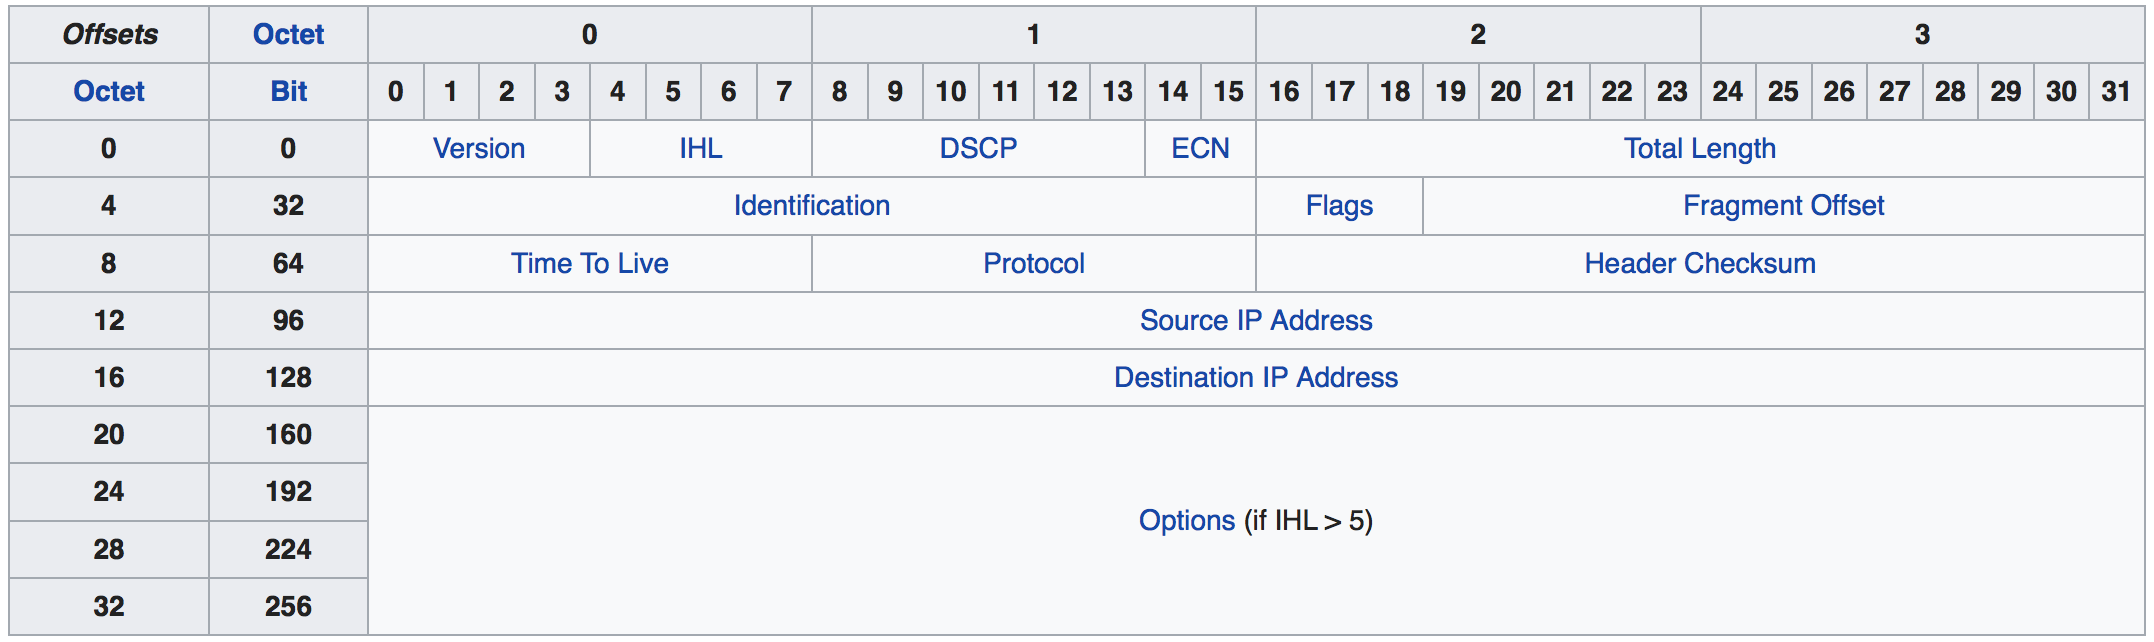
\includegraphics[width=\linewidth]{ipv4}
\end{table}
\begin{description}
	\item[Version:] For IPv4, this is always 4
	\item[Internet Header Length(IHL):] Length of the header times 4 (e.g. IHL = 5, header length is $5\times4=20$ bytes. Minimum value is $5$, max is $15$
	\item[Differentiated Services Code Point (DSCP):] Originally ToS, used for DiffServ technologies requiring real-time streaming (e.g. VoIP)
	\item[Explicit Congestion Notification (ECN):] Notifies each end of congestion without dropping packets
	\item[Total Length:] Entire packet size, including header and data. Min is 20, max is 65,535 bytes
	\item[Identification:] Helps identify groups of IP packets that have been fragmented
	\item[Flags:] bit 0: Reserved, must be zero. bit 1: Don't Fragment (DF). bit 2: More Fragments (MF)
	\item[Fragment Offset:] Measured in 8-byte blocks, provides the offset since the original unfragmented IP datagram
	\item[Time To Live (TTL):] Used to make sure the packet doesn't stay in circulation on the Internet
	\item[Protocol:] See Table~\ref{fig:protocols}. If port 53 and protocol is UDP, DNS request most likely
	\item[Header Checksum:] Checksum for the header only, encapsulated protocol must handle incorrect data errors
	\item[Source Address:] IPv4 sender address for the packet
	\item[Destination Address:] IPv4 receiver address for the packet
	\item[Options:] Options field not often used. IHL must include enough width to allocate for options. Options can end with an EOL (End of Options List, 0x00) if it doesn't match up with ending of IHL. Possible options are:
	\begin{description}
		\item[Copied:] (1 bit) Set to 1 if the options need to be copied into all fragments of a fragmented packet
		\item[Option Class:] (2 bits) A general options category. 0 is for ``control'' options, and 2 is for ``debugging and measurement''. 1 and 3 reserved
		\item[Option Number:] (5 bits) Specifies an option
		\item[Option Length:] (8 bits) Indicated the size of the entire option (including this field). This field may not exist for simple options
		\item[Option Data:] (Variable Bits) Option-specific data. This field may not exist for simple options
	\end{description}
\end{description}
\begin{table}[H]
	\centering
	\caption{Internet Protocol Numbers from RFC 790}\label{fig:protocols}
	\begin{tabular}{rrl}
	\toprule
	Decimal & Hex & Protocol\\
	\midrule
	1 && Internet Control Message Protocol (ICMP)\\
	2 && Internet Group Management Protocol (IGMP)\\
	6 && Transmission Control Protocol (TCP)\\
	17 && User Datagram Protocol (UDP)\\
	41 && IPv6 encapsulation (ENCAP)\\
	89 && Open Shortest Path First (OSPF)\\
	132 && Stream Control Transmission Protocol (SCTP)\\
	\bottomrule
	\end{tabular}
\end{table}

\subsection{Link Layer}
% Ethernet
\begin{figure}[H]
	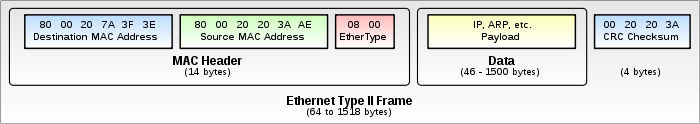
\includegraphics[width=\linewidth]{ethernet}
	\centering
	\caption{Ethernet Breakdown}
\end{figure}
\begin{description}
	\item[Destination:] (6 bytes) Destination MAC Address
	\item[Source:] (6 bytes) Source MAC Address
	\item[Type:] (2 bytes) The type of internet communication (IPv4: 0x0800)
\end{description}
\subsection{Physical}
% Nothing mentioned, just get stuff from notes
	
	\newpage
	\begin{multicols*}{2}
		\section{Protocols}
		% !TeX spellcheck = en_US
% !TeX root = notes.tex
\subsection{Application Layer}
\subsubsection{HTTP: Hypertext Transfer Protocol}
See Section~\ref{sec:http}
\subsubsection{SMTP: Simple Mail Transfer Protocol}
See Section~\ref{sec:smtp}
\subsubsection{DNS: Domain Name Service}
See Section~\ref{sec:dns}
\subsubsection{DASH: Dynamic, Adaptive Streaming over HTTP}
See Section~\ref{sec:dash}

%\subsection{Presentation Layer}
%\subsection{Session Layer}

\subsection{Transport Layer}
\subsubsection{UDP: User Datagram Protocol}
See Section~\ref{sec:udp}
\subsubsection{TCP: Transmission Control Protocol}
See Section~\ref{sec:tcp}
\subsubsection{RTP: Real-Time Protocol}
See Section~\ref{sec:rtp}
\subsubsection{RTCP: Real-Time Control Protocol}
See Section~\ref{sec:rtcp}
\subsubsection{SIP: Session Initiation Protocol}
See Section~\ref{sec:sip}

\subsection{Network Layer}
\subsubsection{IP: Internet Protocol}
See Section~\ref{sec:ip}
\subsubsection{DHCP: Dynamic Host Configuration Protocol}
See Section~\ref{sec:dhcp}
\subsubsection{NAT: Network Address Translation}
See Section~\ref{sec:nat} (this is a technique that just modifies this layer)
\subsubsection{IPv6}
See Section~\ref{sec:ipv6}
\subsubsection{ICMP: Internet Control Message Protocol}
See Section~\ref{sec:icmp}
\subsubsection{OSPF: Open Shortest Path First}
See Section~\ref{note:ospf}\\
Intra-AS Routing, Link-State
\subsubsection{BGP: Border Gateway Protocol}
See Section~\ref{note:bgp}\\
Inter-AS Routing, Distance Vector (Path Vector Protocol)
\subsubsection{IS-IS: Intermediate System to Intermediate System}
Intra-AS Routing, Link-State
\subsubsection{RIP: Routing Information Protocol}
Intra-AS Routing, Distance Vector
\subsubsection{IGRP: Interior Gateway Routing Protocol}
Intra-AS Routing, Distance Vector

\subsection{Link Layer}
\subsubsection{TDMA: Time Division Multiple Access}
See Section~\ref{sec:tdma}
\subsubsection{FDMA: Frequency Division Multiple Access}
See Section~\ref{sec:fdma}
\subsubsection{Slotted ALOHA}
See Section~\ref{sec:saloha}
\subsubsection{Pure (unslotted) ALOHA}
See Section~\ref{sec:paloha}
\subsubsection{CSMA (Carrier Sense Multiple Access)}
See Section~\ref{sec:CSMA}
\subsubsection{CSMA/CD: Collision Detection}
See Section~\ref{sec:CSMA/CD}
\subsubsection{Polling}
See Section~\ref{sec:polling}
\subsubsection{Token Passing}
See Section~\ref{sec:token}
\subsubsection{DOCSIS: Data Over Cable Service Interface Spec}
See Section~\ref{sec:docsis}
\subsubsection{ARP: Address Resolution Protocol}
See Section~\ref{sec:arp}
	\end{multicols*}
	
	\newpage
	\begin{multicols*}{2}
	\section{Acronyms}
	% !TeX spellcheck = en_US
% !TeX root = notes.tex

\begin{description}
	\item[IP:] Internet Protocol
	\item[TCP:] 
	\item[UDP:] 
	\item[HTTP:] Hypertext Transfer Protocol
	\item[SMTP:] Simple Mail Transfer Protocol
	\item[RDP:]	Remote Desktop Protocol
	\item[VOIP:] Voice over IP
	\item[RTT:]
	\item[POP:] Post Office Protocol
	\item[IMAP:] Internet Mail Access Procotol
	\item[DNS:] Domain Name System
	\item[SSN:]
	\item[TLD:] Top-level Domain
	\item[TTL:] Time To Live
	\item[RR:] Resource Records
	\item[DDoS:]
	\item[CBR:] Constant bit rate
	\item[VBR:] Variable bit rate
	\item[ABR:]
	\item[UBR:]
	\item[DASH:] Dynamic, Adaptive Streaming over HTTP
	\item[CDN:] Content Distribution Networks
	\item[RDT:] Reliable Data Transfer
	\item[MSS:]
	\item[ECN:] Explicit Congestion Notification
	\item[ECE:]
	\item[SDN:] Software-defined networking
	\item[TCAMs:] Ternary Content Addressable Memories
	\item[HOL:] Head-of-the-Line
	\item[FIFO:] First in first out
	\item[RR:] Round Robin
	\item[WFQ:] Weighted Fair Queuing
	\item[CIDR:] Classless InterDomain Routing
	\item[DHCP:] Dynamic Host Configuration Protocol
	\item[ICANN:] Internet Corporation for Assigned Names and Numbers
	\item[NAT:] Network Address Translation
	\item[QoS:]
	\item[OSPF:]
	\item[ODL:]
	\item[ONOS:]
	\item[ICMP:] Internet Control Message Protocol
	\item[SNMP:]
	\item[CA:] Control Agent
	\item[DV:] Distance Vector
	\item[B-F:] Bellman-Ford
	\item[LS:] Link State
	\item[AS:] Autonomous Systems
	\item[IGP:] Interior Gateway Protocols
	\item[RIP:] Routing Information Protocol
	\item[OSPF:] Open Shortest Path First
	\item[IGRP:] Interior Gateway Routing Protocol
	\item[ToS:]
	\item[MOSPF:] Multicast OSPF
	\item[BGP:] Border Gateway Protocol
	\item[SDN:] Software Defined Networking
	\item[SNMP:]
	\item[ODL:] OpenDaylight
	\item[SAL:] Service Abstraction Layer
	\item[OVSDB:]
	\item[MIB:] Management Information Base
\end{description}
\end{multicols*}

\newpage
\section{2017 solutions}
\subsection{Question 1}
\begin{figure}[H]
	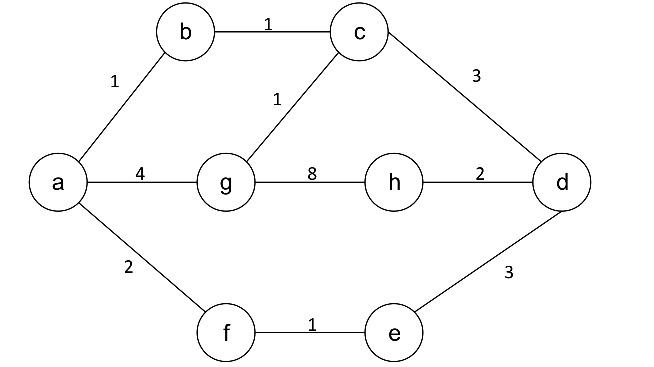
\includegraphics[width=\linewidth]{q1}
\end{figure}
\begin{table}[H]
	\centering
	\caption{Dijkstra's method}
	\rowcolors{2}{gray!25}{white}
	\begin{tabular}{lrrrrrrrr}
		\toprule
		Step &       N' & D(a),p(a) & D(b),p(b) & D(c),p(c) & D(d),p(d) & D(e),p(e) & D(f),p(f) & D(h),p(h) \\ \midrule
		0    &        g &       4,g &  $\infty$ &       1,g &  $\infty$ &  $\infty$ &  $\infty$ &       8,g \\
		1    &       gc &       4,g &       2,c &       1,g &       4,c &  $\infty$ &  $\infty$ &       8,g \\
		2    &      gcb &       3,b &       2,c &           &       4,c &  $\infty$ &  $\infty$ &       8,g \\
		3    &     gcba &       3,b &           &           &       4,c &  $\infty$ &       5,a &       8,g \\
		4    &    gcbaf &           &           &           &       4,c &       6,f &       5,a &       8,g \\
		5    &   gcbafe &           &           &           &       4,c &       6,f &           &       8,g \\
		6    &  gcbafed &           &           &           &       4,c &           &           &       6,d \\
		7    & gcbafedh &           &           &           &           &           &           &       6,d \\
		8    &          &           &           &           &           &           &           &
	\end{tabular}
\end{table}
\begin{table}[H]
	\begin{tabular}{lll}
		\toprule
		From node g to & Minimum Path & Minimum Distance \\ \midrule
		a              & gcba         & 3                \\
		b              & gcb          & 2                \\
		c              & gc           & 1                \\
		d              & gcd          & 4                \\
		e              & gcbafe       & 6                \\
		f              & gcbaf        & 5                \\
		h              & gcdh         & 6
	\end{tabular}
\end{table}
\begin{figure}[H]
	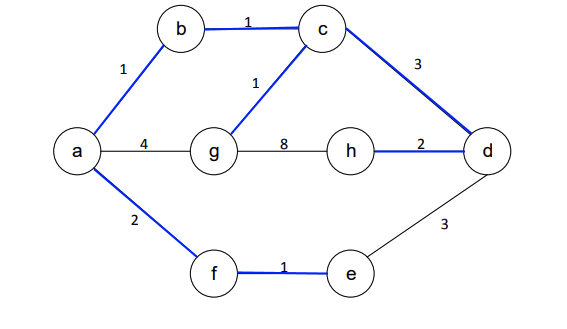
\includegraphics[width=\linewidth]{q1b}
\end{figure}
If output ports from \textbf{g} to nodes \textbf{a}, \textbf{c}, and \textbf{h} are called `ga', `gc', and `gh' respectively, show a forwarding table, based on the above minimum paths, which shows the output links from g for all destination nodes
\begin{table}[H]
	\centering
	\begin{tabular}{lc}
		\toprule
		List of destination nodes & To be sent over link\\
		\midrule
		None (other routes faster) & ga\\
		All (quickest routes for all) & gc\\
		Non (other routes faster) & gh
	\end{tabular}
\end{table}
\subsection{Question 2}
\begin{table}[H]
	\centering
	\begin{tabular}{p{10cm}ll}
		\toprule
		Purpose of this Protocol                                                        & Name           & Layer       \\ \midrule
		Example: Retrieve web pages                                                     & HTTP           & Application \\
		Convey network management control and information messages                      & SNMP           & Application \\
		Send email message to a mail server                                             & SMTP           & Application \\
		Download email messages from a mail server                                      & IMAP/POP3      & Application \\
		``Ping'' a host                                                                 & IMCP           & Network     \\
		Convert a hostname to an IP address                                             & DNS            & Application \\
		Convert an IP address to a MAC address                                          & ARP            & Link        \\
		Sending intra-AS link-state routing messages                                    & OSPF/IS-IS     & Network     \\
		Setting up multimedia stream connections                                        & SIP            & Transport   \\
		Providing connectivity between hosts and access points in WiFi networks         & 802.11         & Physical    \\
		An enhanced version of connection-oriented stream transport which adds security & QUIC (TLS/SSL) & Application
	\end{tabular}
\end{table}
\subsection{Question 3}
TCP packet inside an IP packet inside Ethernet frame (preamble and CRC)\\
\texttt{aa aa aa aa aa aa aa ab}\qquad \texttt{00 00 5e 00 01 08 98 90}\\
\texttt{96 d8 35 a9 08 00 45 00\qquad 00 28 41 71 40 00 80 06}\\
\texttt{00 00 0a 21 02 98 d0 5c\qquad ec 52 e1 75 00 50 e7 3e}\\
\texttt{50 0c 1b a0 80 d4 50 11\qquad f7 39 c9 82 00 00 00 00}\\
\texttt{00 00 00 00 c8 aa ab cd}\\
IP is 40 bytes long\\
\begin{table}[H]
	\begin{tabular}{ll}
		\toprule
		Field                        & (Format) Value                                           \\ \midrule
		Ethernet Source Address      & (Hexadecimal) 98:90:96:d8:35:a9                          \\
		Ethernet Destination Address & (Hexadecimal) 00:00:5e:00:01:08                          \\
		IP Source Address            & (Dotted Decimal) 0a 21 02 98 $\rightarrow$ 10.33.2.152   \\
		IP Destination Address       & (Dotted Decimal) d0 5c ec 52 $\rightarrow$ 208.92.236.82 \\
		TCP Source Port              & (Decimal) e1 75 $\rightarrow$ 57717                      \\
		TCP Destination Port         & (Decimal) 00 50 $\rightarrow$ 80                         \\
		IP Version                   & (Decimal) 4                                              \\
		IP Header Length in bytes    & (Decimal) 20                                             \\
		IP Datagram Length in bytes  & (Decimal) 28                                              \\
		TCP Flags                    & (Binary) URG: 0                                          \\
		                             & (Binary) ACK: 1                                          \\
		                             & (Binary) PSH: 0                                          \\
		                             & (Binary) RST: 0                                          \\
		                             & (Binary) SYN: 0                                          \\
		                             & (Binary) FIN: 1                                          \\
		TCP Sequence Number          & (Hex) e7 3e 50 0c                                        \\
		TCP Acknowledgment Number    & (Hex) 1b a0 80 d4                                        \\
		IP Header Checksum           & (Hex) 00 00                                              \\
		TCP Internet Checksum        & (Hex) c9 82                                              \\
		Ethernet CRC                 & (Hex) ab cd
	\end{tabular}
\end{table}
\subsection{Question 4}
\subsubsection{Link-state and distance-vector}
Distance-vector, each node tells its neighbors everything it knows about the network. In Link-State, each router broadcasts the state of its own links to the entire network. Leaving each router to build up a graph of the network. LS has the advantage that is updates router's graphs quicker across the network because it broadcasts changes. DV advantage is that it uses less memory and CPU by not having to build up graphs, only populate a routing table
\subsubsection{Destination-based forwarding and Software-defined-networking}
Destination-based forwarding forwards packets towards their end destination by a routing table of destinations and links. SDN uses a central controller to direct packets using more complex rules than just routing tables. Advantage of destination-based: is that's very simple to implement and is self-managing. Advantage of SDN: you can route packets by type of traffic or link cost (peering agreement)
\subsubsection{TCP and UDP}
TCP uses a 3-way handshake to open a `connection' between hosts, and within that connection, packets are guaranteed to arrive eventually. UDP packets are send off and forgotten about, and may not arrive. TCP advantage: IP address can not be spoofed. UDP advantage: save the overhead dealing with connections for simple messages or real-time applications
\subsubsection{Go-Back-N and Selective-Repeat}
GBN will retransmit all the packets after the last successful ACK that timed out, whereas SR will only retransmit the lost packets that weren't ACK'd. GBN advantage is it doesn't need to ACK every single packet, just every X number. SR saves retransmitting even correctly received packet


\end{document}